% mnras_template.tex 
%
% LaTeX template for creating an MNRAS paper
%
% v3.0 released 14 May 2015
% (version numbers match those of mnras.cls)
%
% Copyright (C) Royal Astronomical Society 2015
% Authors:
% Keith T. Smith (Royal Astronomical Society)

% Change log
%
% v3.0 May 2015
%    Renamed to match the new package name
%    Version number matches mnras.cls
%    A few minor tweaks to wording
% v1.0 September 2013
%    Beta testing only - never publicly released
%    First version: a simple (ish) template for creating an MNRAS paper

%%%%%%%%%%%%%%%%%%%%%%%%%%%%%%%%%%%%%%%%%%%%%%%%%%
% Basic setup. Most papers should leave these options alone.
\documentclass[fleqn,usenatbib]{mnras}

% MNRAS is set in Times font. If you don't have this installed (most LaTeX
% installations will be fine) or prefer the old Computer Modern fonts, comment
% out the following line
\usepackage{newtxtext,newtxmath}
% Depending on your LaTeX fonts installation, you might get better results with one of these:
%\usepackage{mathptmx}
%\usepackage{txfonts}

% Use vector fonts, so it zooms properly in on-screen viewing software
% Don't change these lines unless you know what you are doing
\usepackage[T1]{fontenc}

% Allow "Thomas van Noord" and "Simon de Laguarde" and alike to be sorted by "N" and "L" etc. in the bibliography.
% Write the name in the bibliography as "\VAN{Noord}{Van}{van} Noord, Thomas"
\DeclareRobustCommand{\VAN}[3]{#2}
\let\VANthebibliography\thebibliography
\def\thebibliography{\DeclareRobustCommand{\VAN}[3]{##3}\VANthebibliography}


%%%%% AUTHORS - PLACE YOUR OWN PACKAGES HERE %%%%%

% Only include extra packages if you really need them. Common packages are:
\usepackage{graphicx}	% Including figure files
\usepackage{amsmath}	% Advanced maths commands
% \usepackage{amssymb}	% Extra maths symbols

\usepackage[dvipsnames]{xcolor}

%%%%%%%%%%%%%%%%%%%%%%%%%%%%%%%%%%%%%%%%%%%%%%%%%%

%%%%% AUTHORS - PLACE YOUR OWN COMMANDS HERE %%%%%

% Please keep new commands to a minimum, and use \newcommand not \def to avoid
% overwriting existing commands. Example:
%\newcommand{\pcm}{\,cm$^{-2}$}	% per cm-squared

\newcommand{\todo}[1]{\textcolor{Magenta}{\textbf{Address: #1}}}
\newcommand{\atsameer}[1]{\textcolor{CornflowerBlue}{\textbf{@Sameer or Jane: #1}}}
\newcommand{\atcameron}[1]{\textcolor{BurntOrange}{\textbf{@Cameron: #1}}}
\newcommand{\atnastasha}[1]{\textcolor{Plum}{\textbf{@Nastasha: #1}}}
\newcommand{\atnir}[1]{\textcolor{ForestGreen}{\textbf{@Nir: #1}}}




%%%%%%%%%%%%%%%%%%%%%%%%%%%%%%%%%%%%%%%%%%%%%%%%%%

%%%%%%%%%%%%%%%%%%% TITLE PAGE %%%%%%%%%%%%%%%%%%%

% Title of the paper, and the short title which is used in the headers.
% Keep the title short and informative.
\title[Halo21 CGM Modeling Challenge]{The Halo21 Absorption Modeling Challenge: [Takeaway Title Message Here]}

% The list of authors, and the short list which is used in the headers.
% If you need two or more lines of authors, add an extra line using \newauthor
\author[]{
The Halo 21 Absorption Modeling Group
\\
% List of institutions
$^{1}$TBD\\
}

% These dates will be filled out by the publisher
\date{Accepted XXX. Received YYY; in original form ZZZ}

% Enter the current year, for the copyright statements etc.
\pubyear{2015}

% Don't change these lines
\begin{document}
\label{firstpage}
\pagerange{\pageref{firstpage}--\pageref{lastpage}}
\maketitle

% Abstract of the paper
\begin{abstract}
This is a simple template for authors to write new MNRAS papers.
The abstract should briefly describe the aims, methods, and main results of the paper.
It should be a single paragraph not more than 250 words (200 words for Letters).
No references should appear in the abstract.
\end{abstract}

% Select between one and six entries from the list of approved keywords.
% Don't make up new ones.
\begin{keywords}
keyword1 -- keyword2 -- keyword3
\end{keywords}

%%%%%%%%%%%%%%%%%%%%%%%%%%%%%%%%%%%%%%%%%%%%%%%%%%

%%%%%%%%%%%%%%%%% BODY OF PAPER %%%%%%%%%%%%%%%%%%
\section{NOTES FOR AUTHORS}

\subsection{KEY FOR COAUTHORS}

\textbf{Bold: Notes for things to implement.}
\textit{Italics: Rough text, needs polishing.}
Normal: Normal text, polished enough to be included in a draft.

\subsection{Outstanding Questions/Discussion Points}

% Who is the target audience?
\textbf{Who is the target audience?}
Imagine sitting down with the target audience.
What are the most important points we want to convey?
In particular, what could they really use?

\section{Introduction}

% Other mock data challenges
Other mock data challenges include a mock data challenge for detecting a gravitational-wave background~\cite{Meacher2015}, a mock data challenge for discriminating overlapping gravitational-wave signals~\cite{Regimbau2012},  and a mock data challenge for identifying gravitational-wave signals in pulsar timing array data~\cite{Hazboun2019}.
\todo{What other mock data challenges are there?}

% Mock CGM analyses of robustness of modeling.
\cite{Liang2018} determined that a Bayesian method of modeling absorption lines was able to derive LOS mass-weighted properties.
\cite{Marra2021} confirmed this finding using a blind study of spectra from cosmological simulations of a $z=1$ Milky Way-type galaxy and a $z=0$ dwarf galaxy.
\cite{Acharya2021} test the robustness of density and metallicity to changes in the UV background, and find that these quantities are uncertain by factors of $\approx 4-6.3$ and $\approx 1.6-3.2$ respectively.
\todo{What other similar studies are there?}
\todo{What else can we learn from these studies?}

\todo{Add a paragraph describing how the challenge was set up.}

\section{Synthetic Data Generation}

% Summary
Data generators produced three mock data samples of increasing sophistication for observers to model:
a highly-idealized sample consisting of ion column densities for uniform clouds,
a sample consisting of spectra generated with properties drawn from a cosmological simulation,
and a sample of spectra drawn directly from a high-resolution simulation.

% Spectra generation
The synthetic spectrum generator \textsc{trident} was used during the production of all three samples.
\atcameron{
Would you mind adding a summary paragraph of Trident here?
}

\subsection{Highly idealized --- \texttt{sample0}}
\label{s: data generation -- sample0}

% Sample summary and motivation
The first data sample, \texttt{sample0} was a highly idealized sample consisting of 10 clouds of uniform metallicity, density, and temperature.
The data products made available to modelers were total ion column densities, as opposed to full spectra.
The motivation for \texttt{sample0} was to set a baseline for interpreting the subsequent data samples, absent complications from multiphase structure or interpreting spectra.

% Sample details
For each of the 10 uniform clouds we sampled from $Z$ = [ 0.01, 1.5 ] $Z_\odot$, $n_{\rm H}$ = [ 10-6, 0.1 ] cm$^{-3}$, $T$ = [ $10^4$, $10^6$ ] K.
The values of density, temperature, and metallicity were chosen to be uncorrelated, which plays a role in the analysis (\S\ref{s: results -- idealized}).
Our mock observing instrument was COS G130M, we set the redshift for our mock sample to $z=0.25$ (typical for many CGM samples observed with COS), and we included all ions present in the instrument window at $z=0.25$~\todo{Mention which ions explicitly.}.
For each ion we looked up the ion densities according to photo-ionization equilibrium, as tabulated by \textsc{trident} for single zone simulations produced with \textsc{cloudy}~\citep{Ferland2013} using the \cite{Haardt2012} UV background.
To determine the absorber lengths ($\ell = N_{\ion{H}{I}} / n_{\ion{H}{I}}$) we randomly sample the \ion{H}{I} column density from $N_{\ion{H}{I}}$ = [ $10^{15}$, $10^{17}$ ] cm$^{-2}$, and discarded absorbers with length $> 1$ Mpc.

% Noising of data
Prior to making the ion column densities available we modified them to reflect uncertainty typical of similar real observations.
\todo{Continue here.}

\subsection{Informed by cosmological simulations  --- \texttt{sample1}}
\label{s: data generation -- sample1}

\textbf{This corresponds to sample1.}

% \atnastasha{
% I have copied in what you wrote about extracting the distributions from the simulations, along with my edited version to fit into the paper.
% Can you please review the edited version for correctness?
% }

\subsection{Drawn from a high resolution simulation --- \texttt{sample2}}
\label{s: data generation -- sample2}

\textbf{This corresponds to sample2.}

% \atnir{
% I have copied in what you wrote about extracting the distributions from the simulations, along with my edited version to fit into the paper.
% Can you please review the edited version for correctness?
% }

% C IV and changed redshift
\textit{
We changed the redshift to $z=0.13$ to bring \ion{C}{IV} into the observable range for the COS gratings.
Note that the simulations were run at $z=2$, including a $z=2$ UVB background.
However, the ionization fractions were calculated in post-processing via Trident using a $z=0.13$ UVB background.
}

\section{Observational Modeling}

\atsameer{
Can you please describe your modeling in this section?
Ideally you would include a short summary of your modeling, accompanied by citations to your paper containing the full details.
}

\section{Results}

\subsection{Highly idealized}
\label{s: results -- idealized}

\begin{figure*}
    \centering
    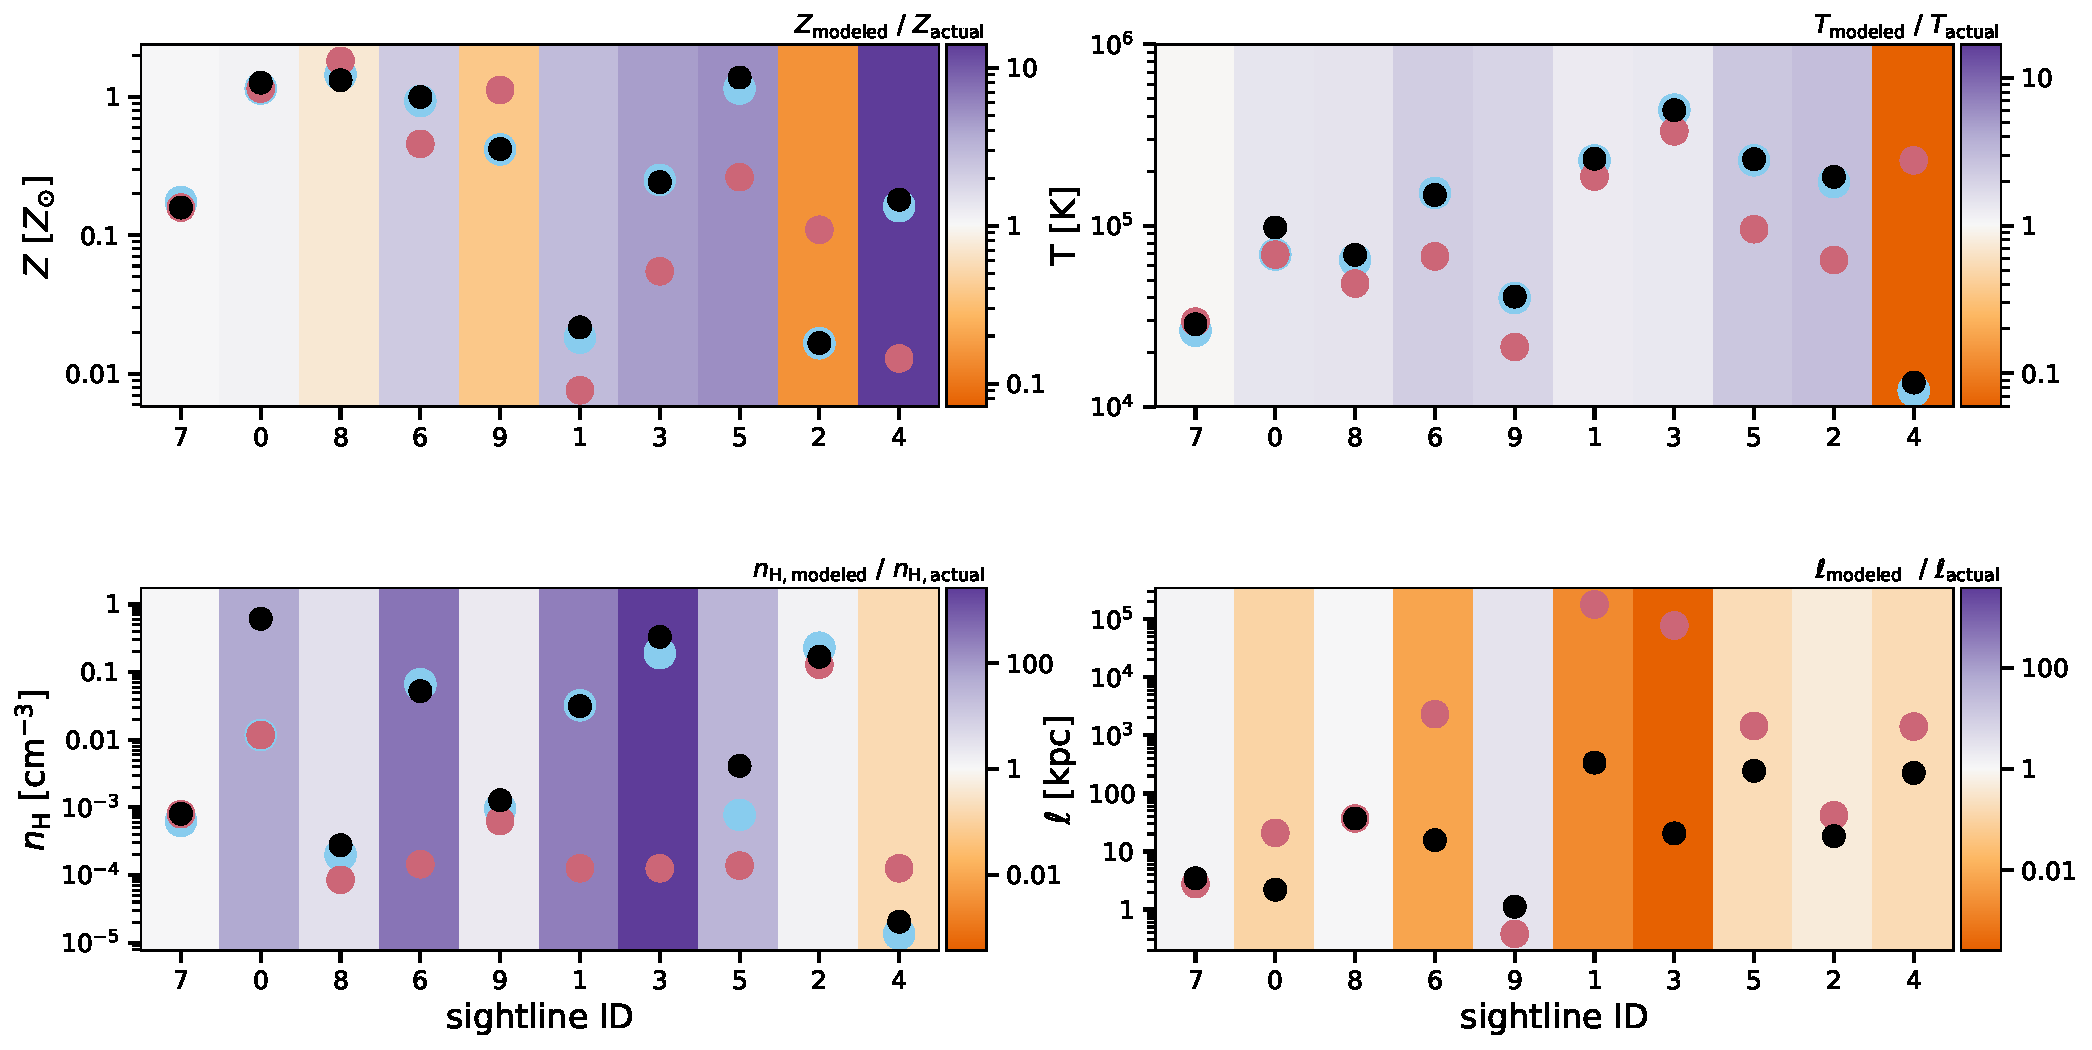
\includegraphics[width=\textwidth]{figures/sample0/comparison.pdf}
    \caption{
    Comparison in highly idealized scenario.
    }
    \label{f: idealized}
\end{figure*}

\begin{figure}
    \centering
    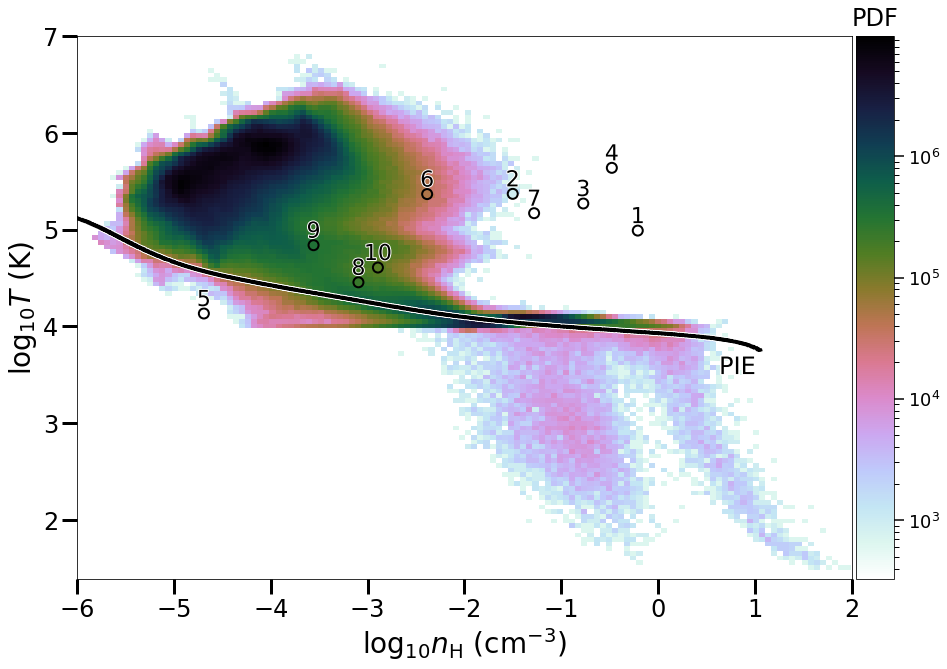
\includegraphics[width=\columnwidth]{figures/sample0/phase_space.png}
    \caption{
    \todo{Set colorbar by percent enclosed.}
    \todo{Use consistent axes: all log, or no log.}
    }
    \label{f: idealized explanation}
\end{figure}

\begin{figure*}
    \centering
    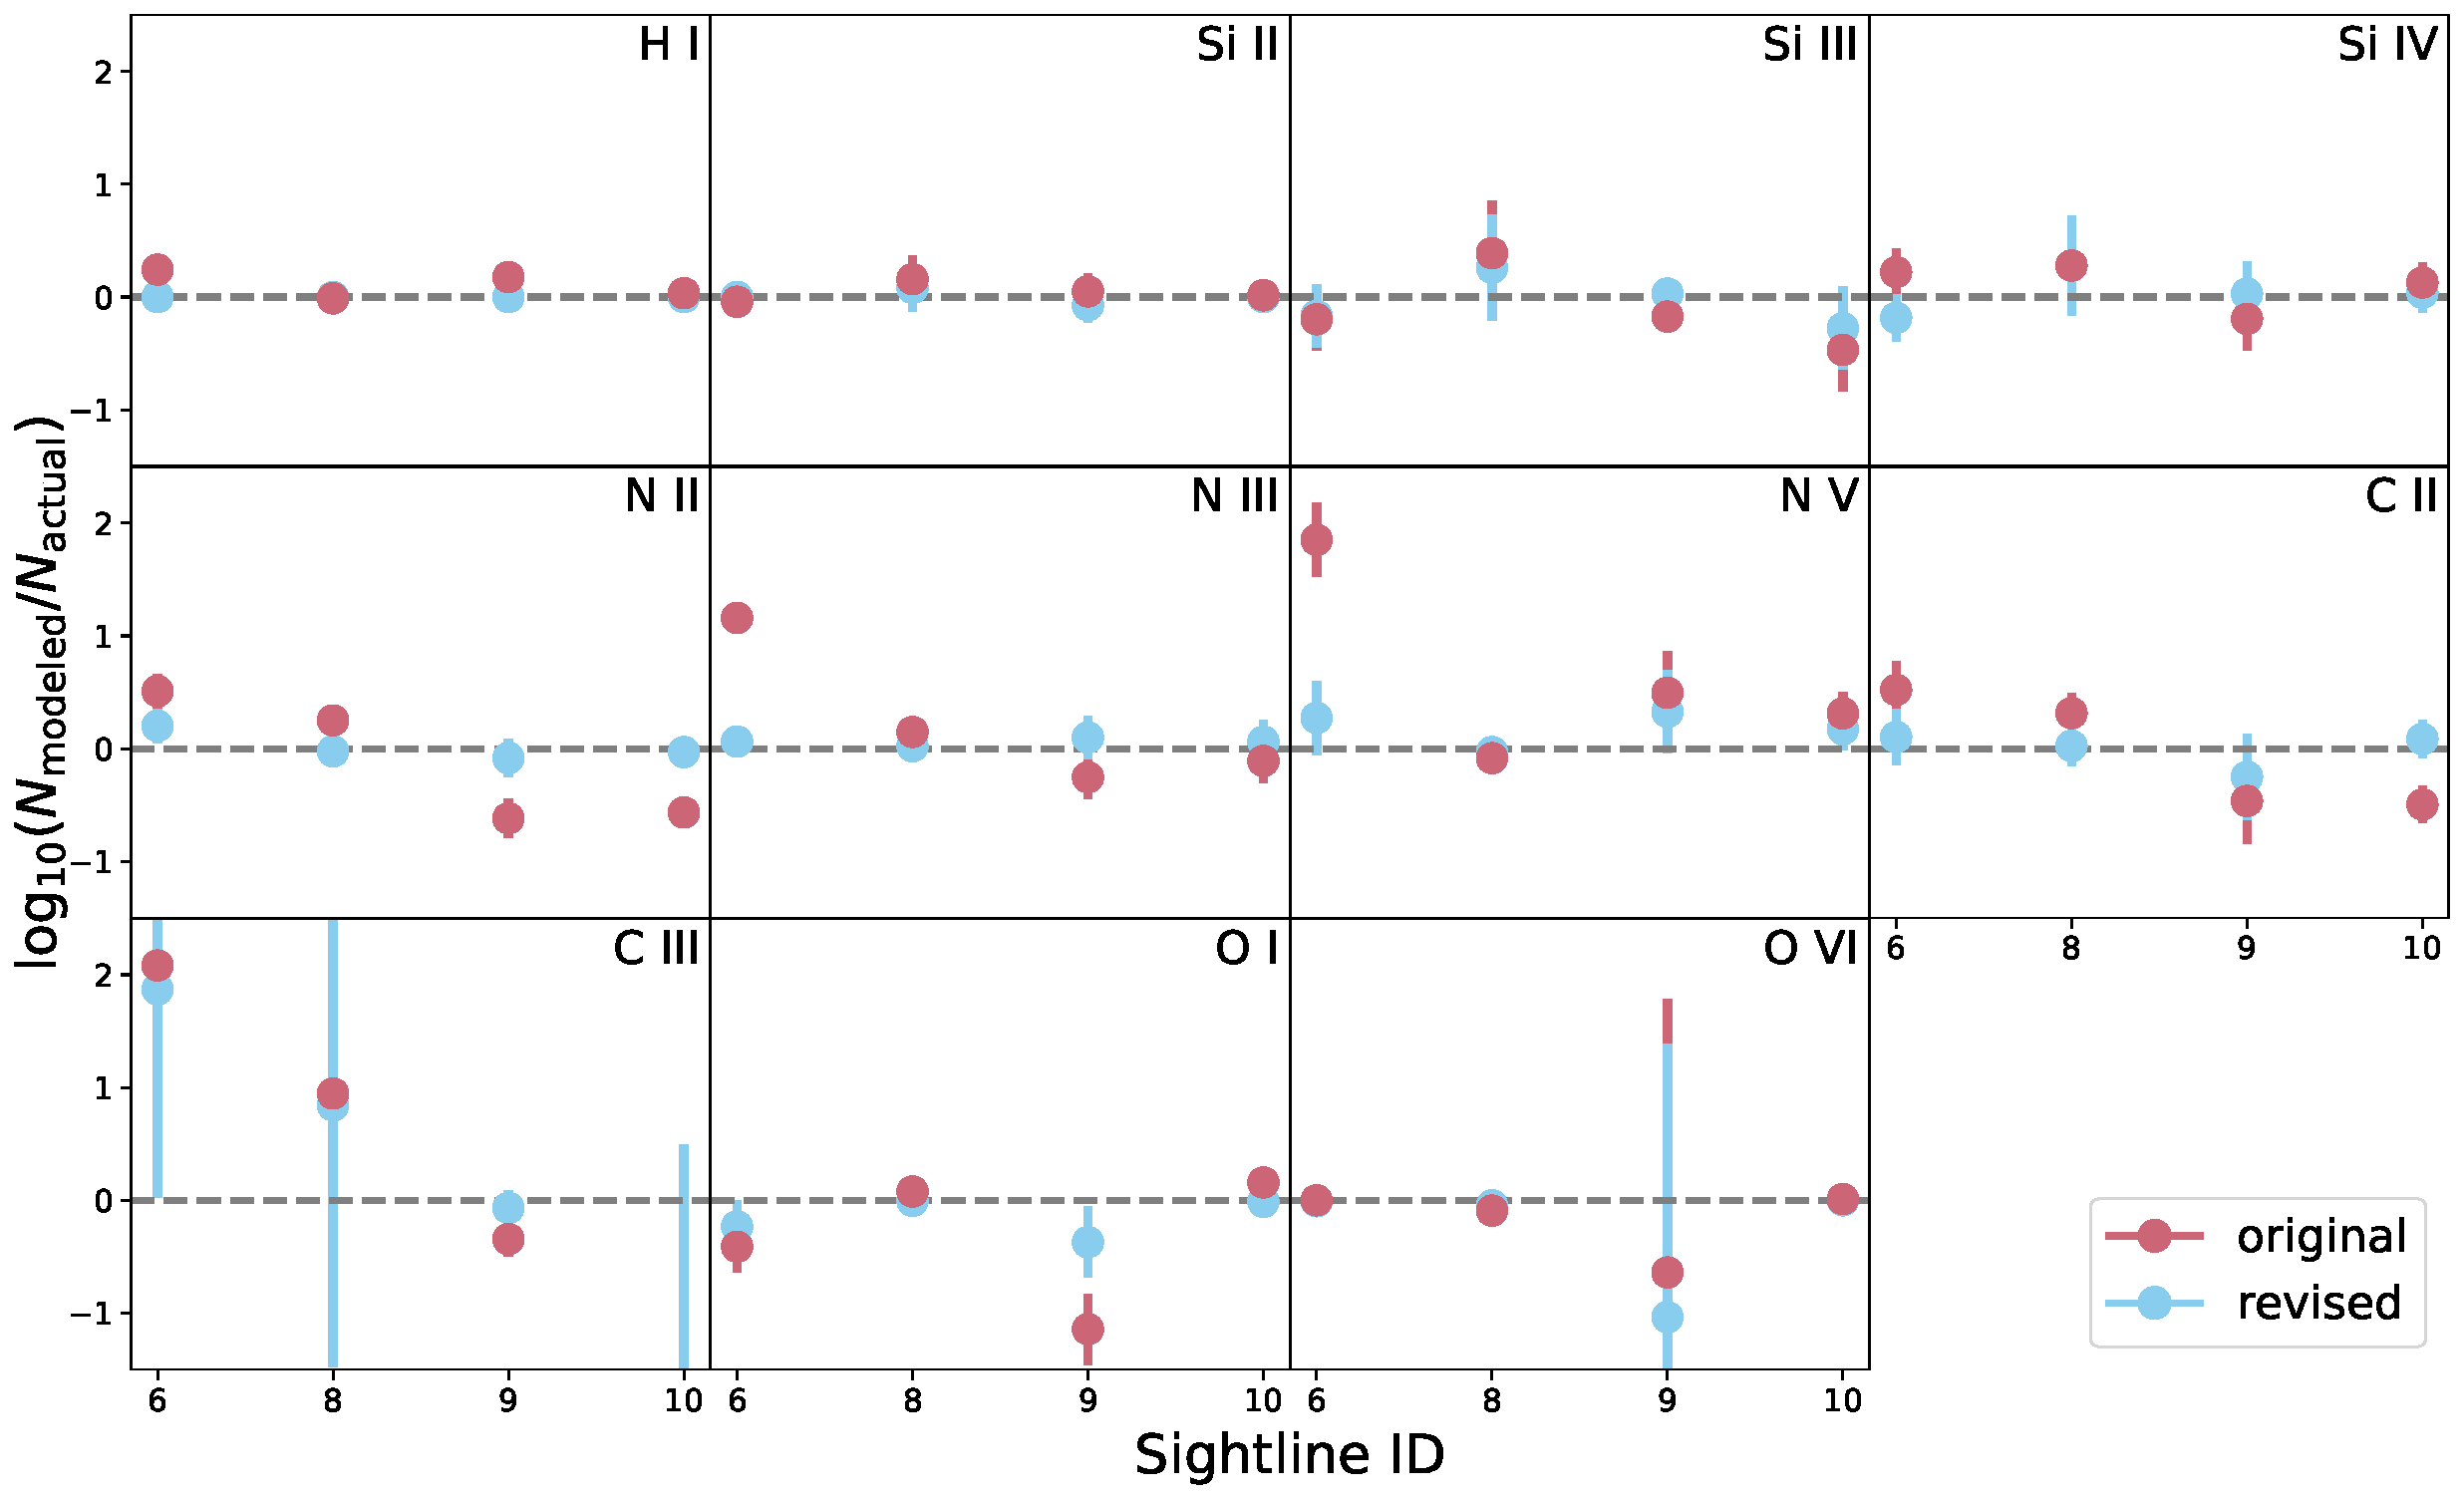
\includegraphics[width=\textwidth]{figures/sample0/column_den.pdf}
    \label{f: column density agreement}
\end{figure*}

\subsection{Informed by cosmological simulations}

\begin{figure}
    \centering
    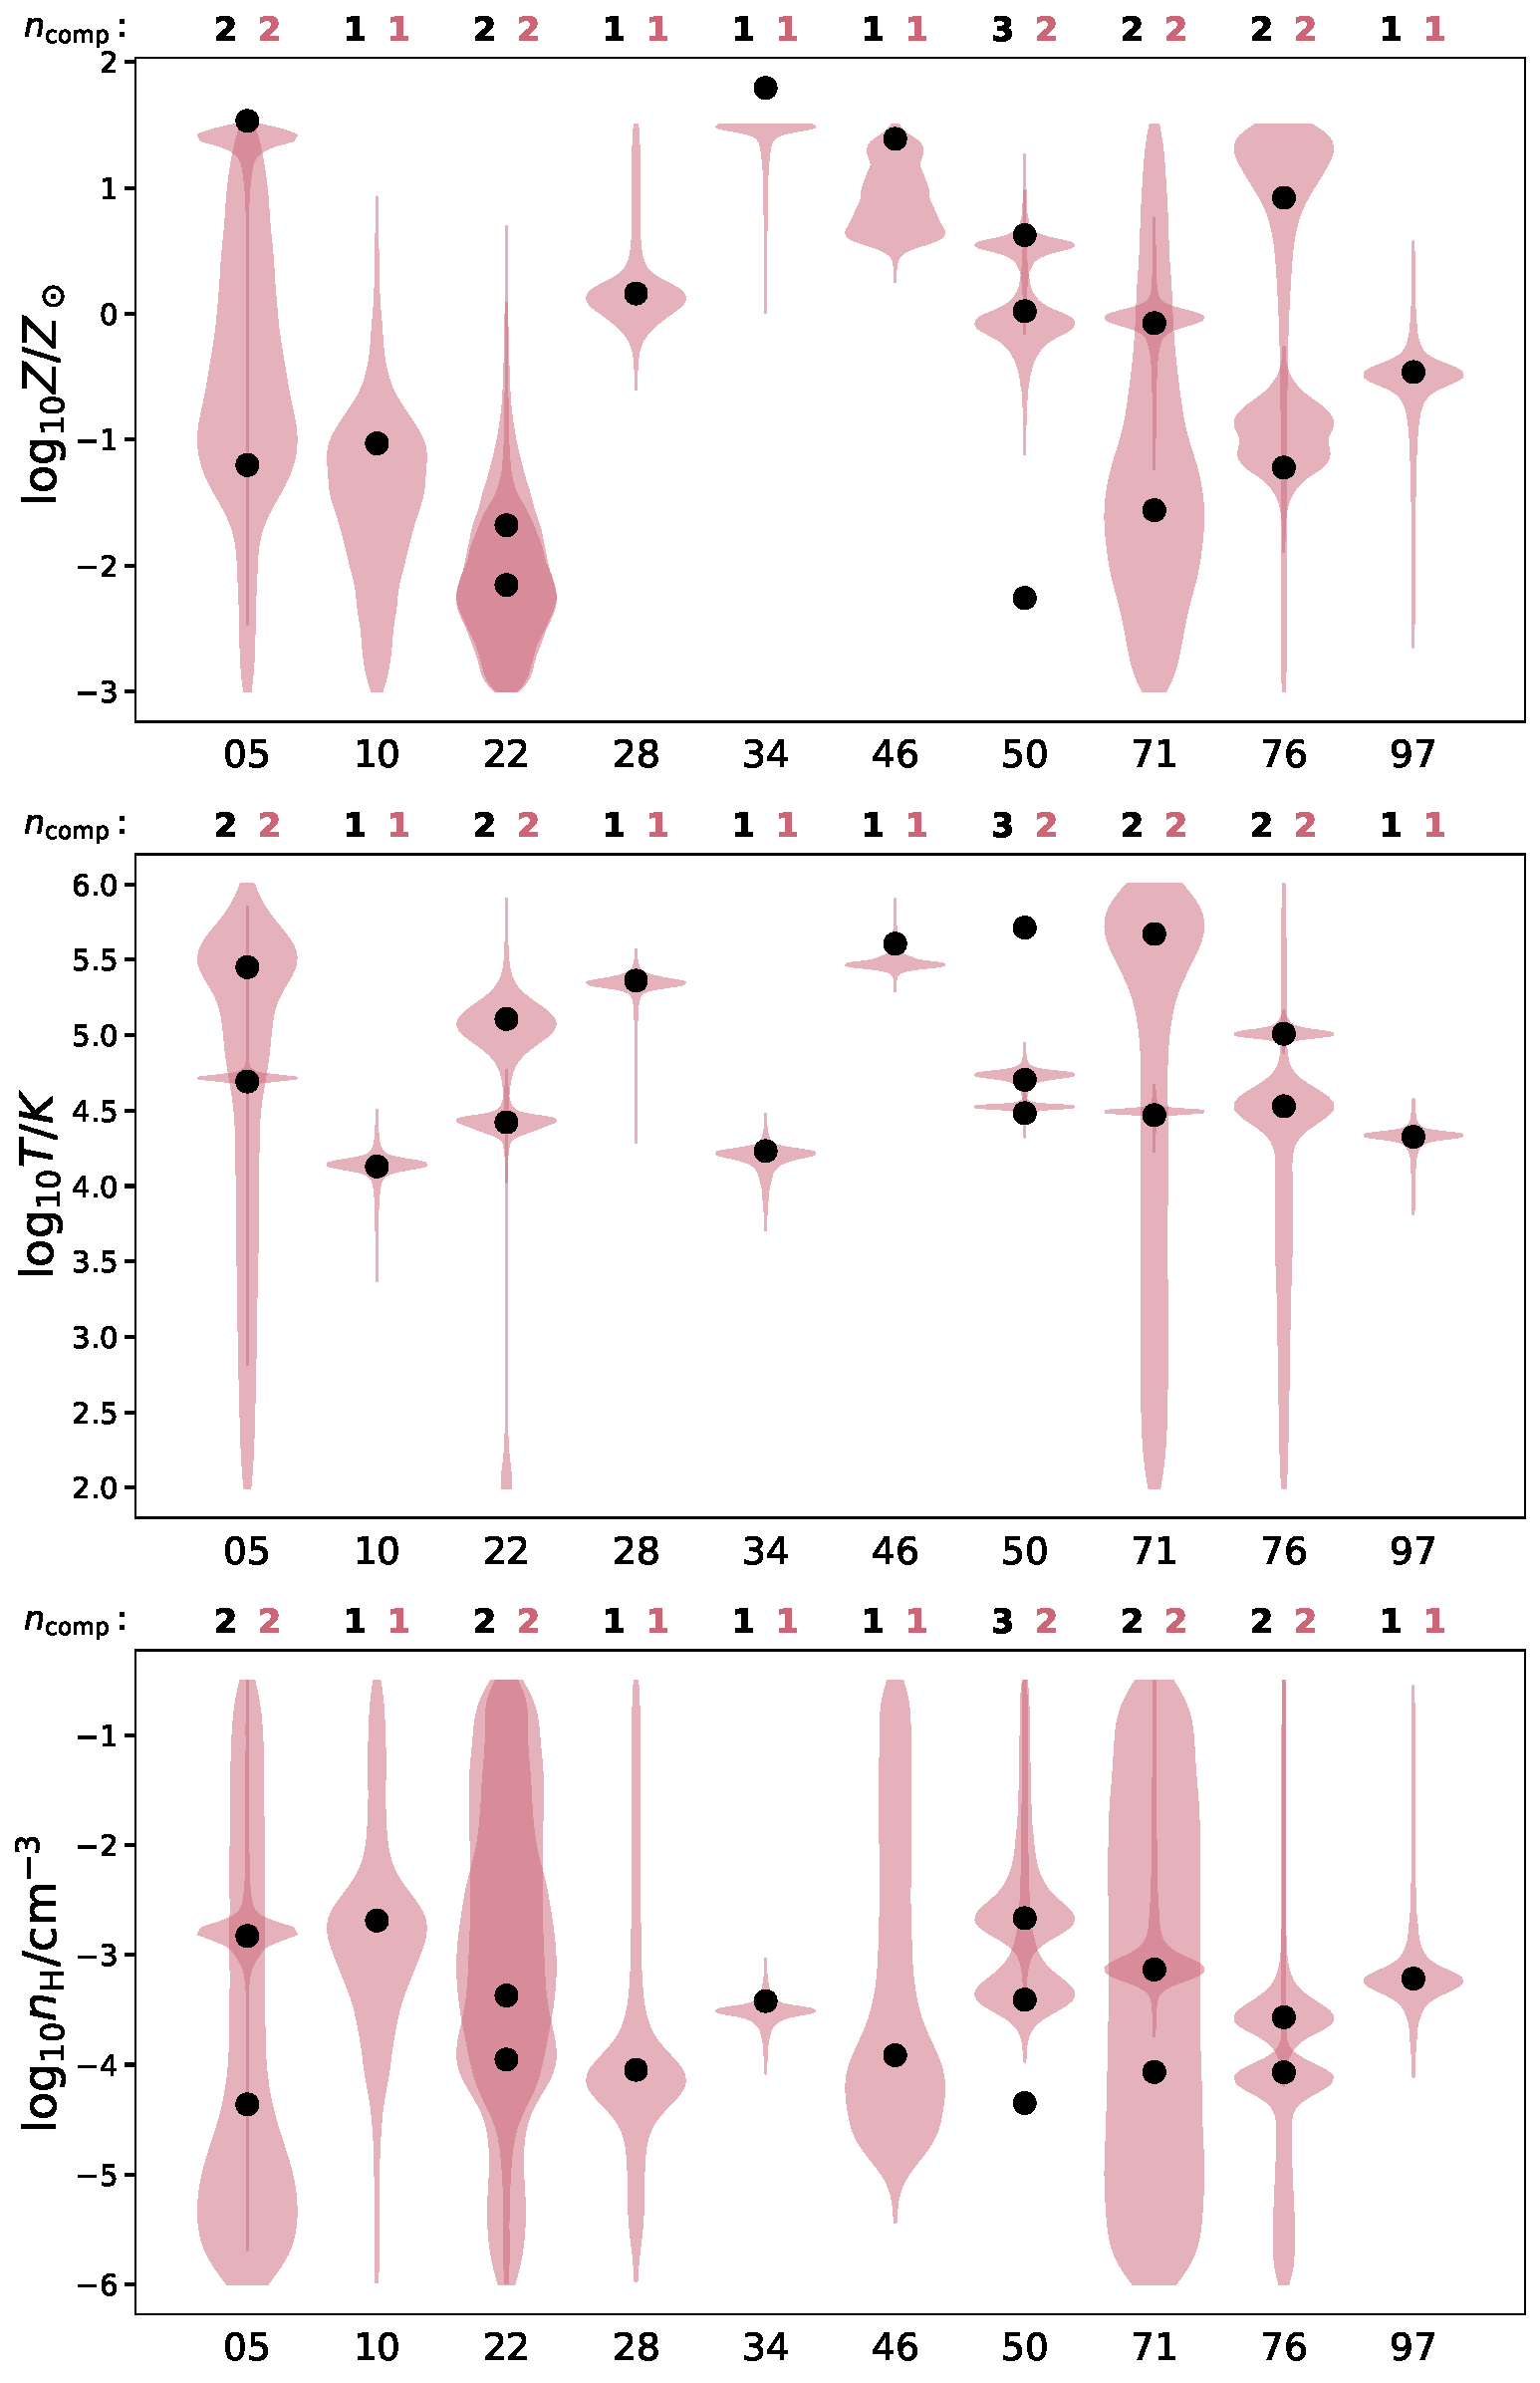
\includegraphics[width=\columnwidth]{figures/sample1/comparison.pdf}
    \caption{
    Comparison informed by cosmological simulations.
    }
    \label{f: informed}
\end{figure}

\subsection{Drawn from high resolution simulations}

\begin{figure*}
    \centering
    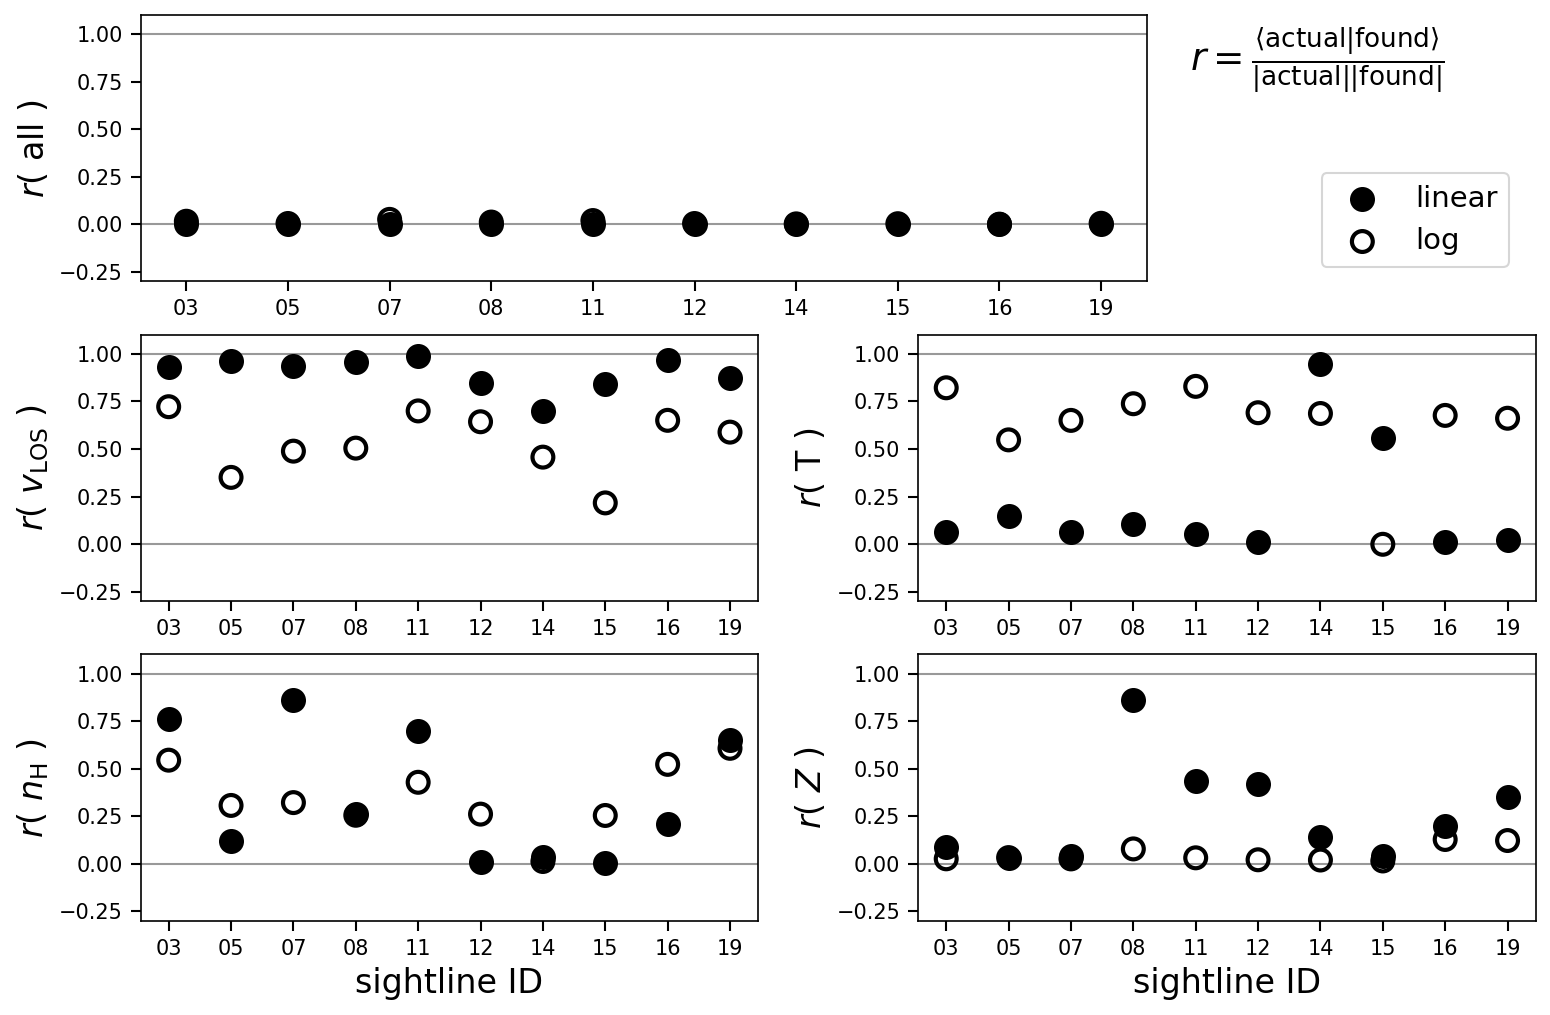
\includegraphics[width=\textwidth]{figures/sample2/correlations.png}
    \label{f: high-res}
    \caption{
    \todo{Use ``modeled'', not ``found''.}
    \todo{Cut out $r( {\rm all} )$.}
    }
\end{figure*}

\begin{figure*}
    \centering
    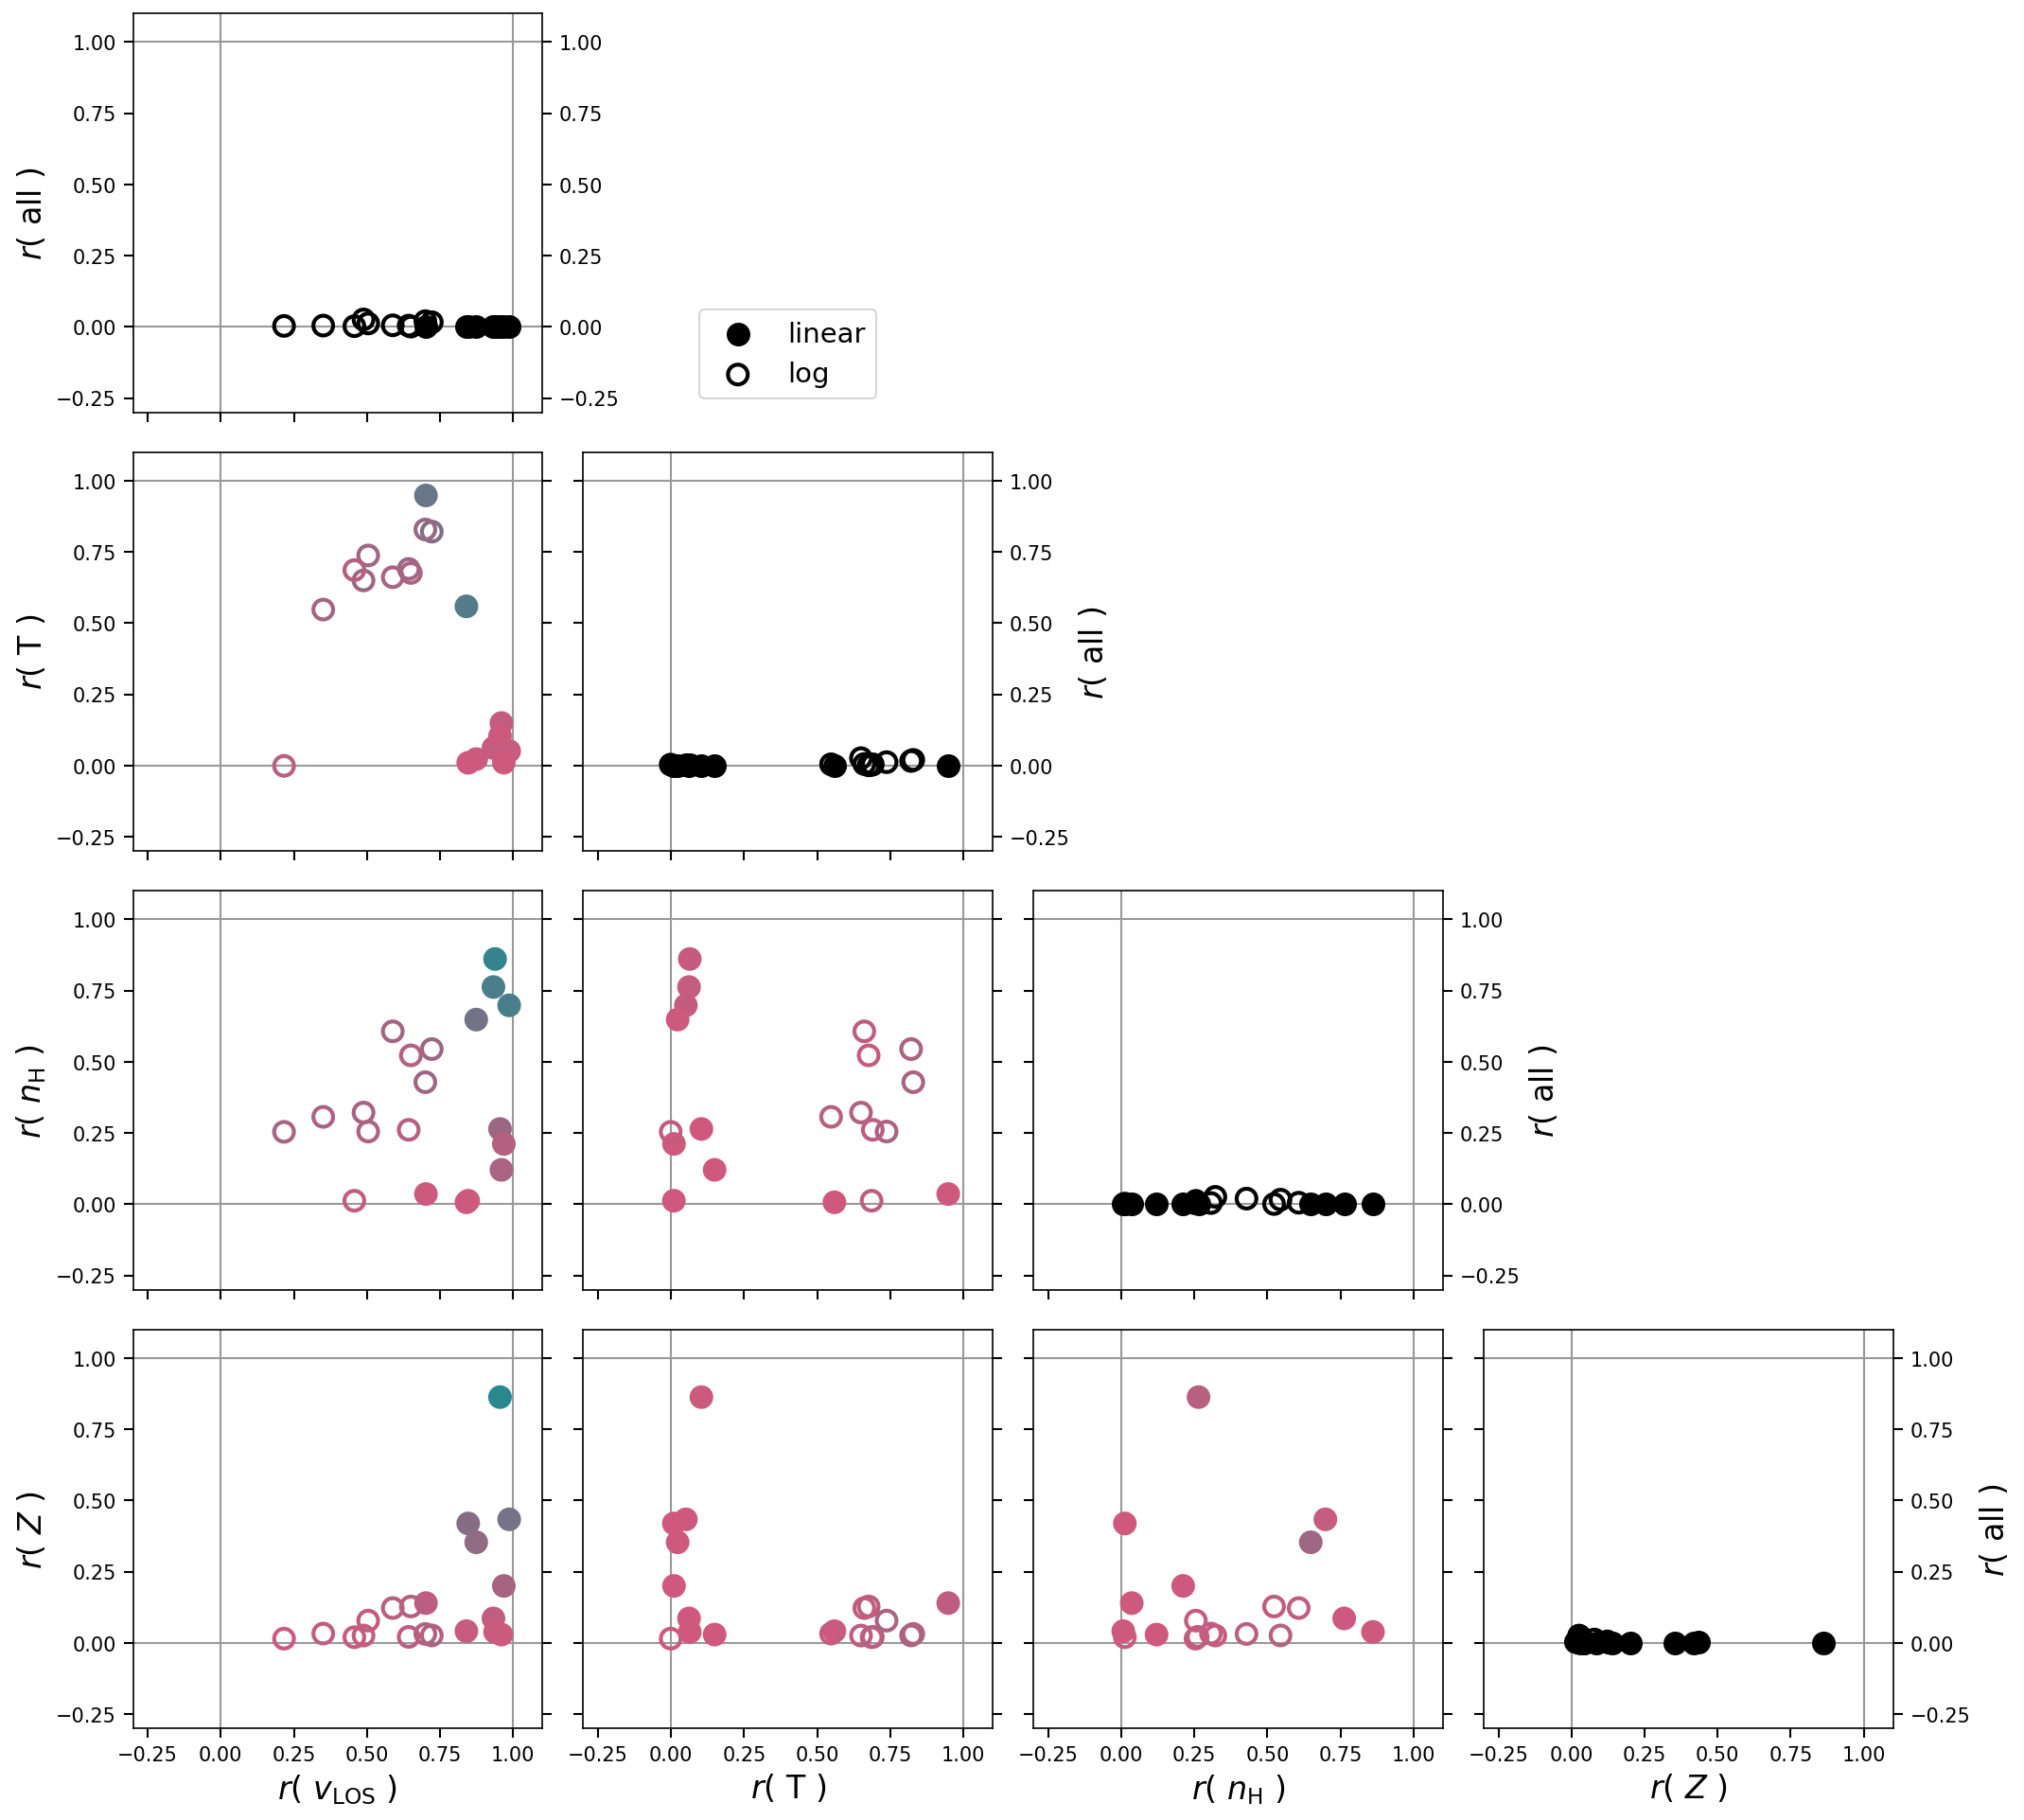
\includegraphics[width=\textwidth]{figures/sample2/correlations_corner.png}
    \label{f: high-res corner}
\end{figure*}

\begin{figure*}
    \centering
    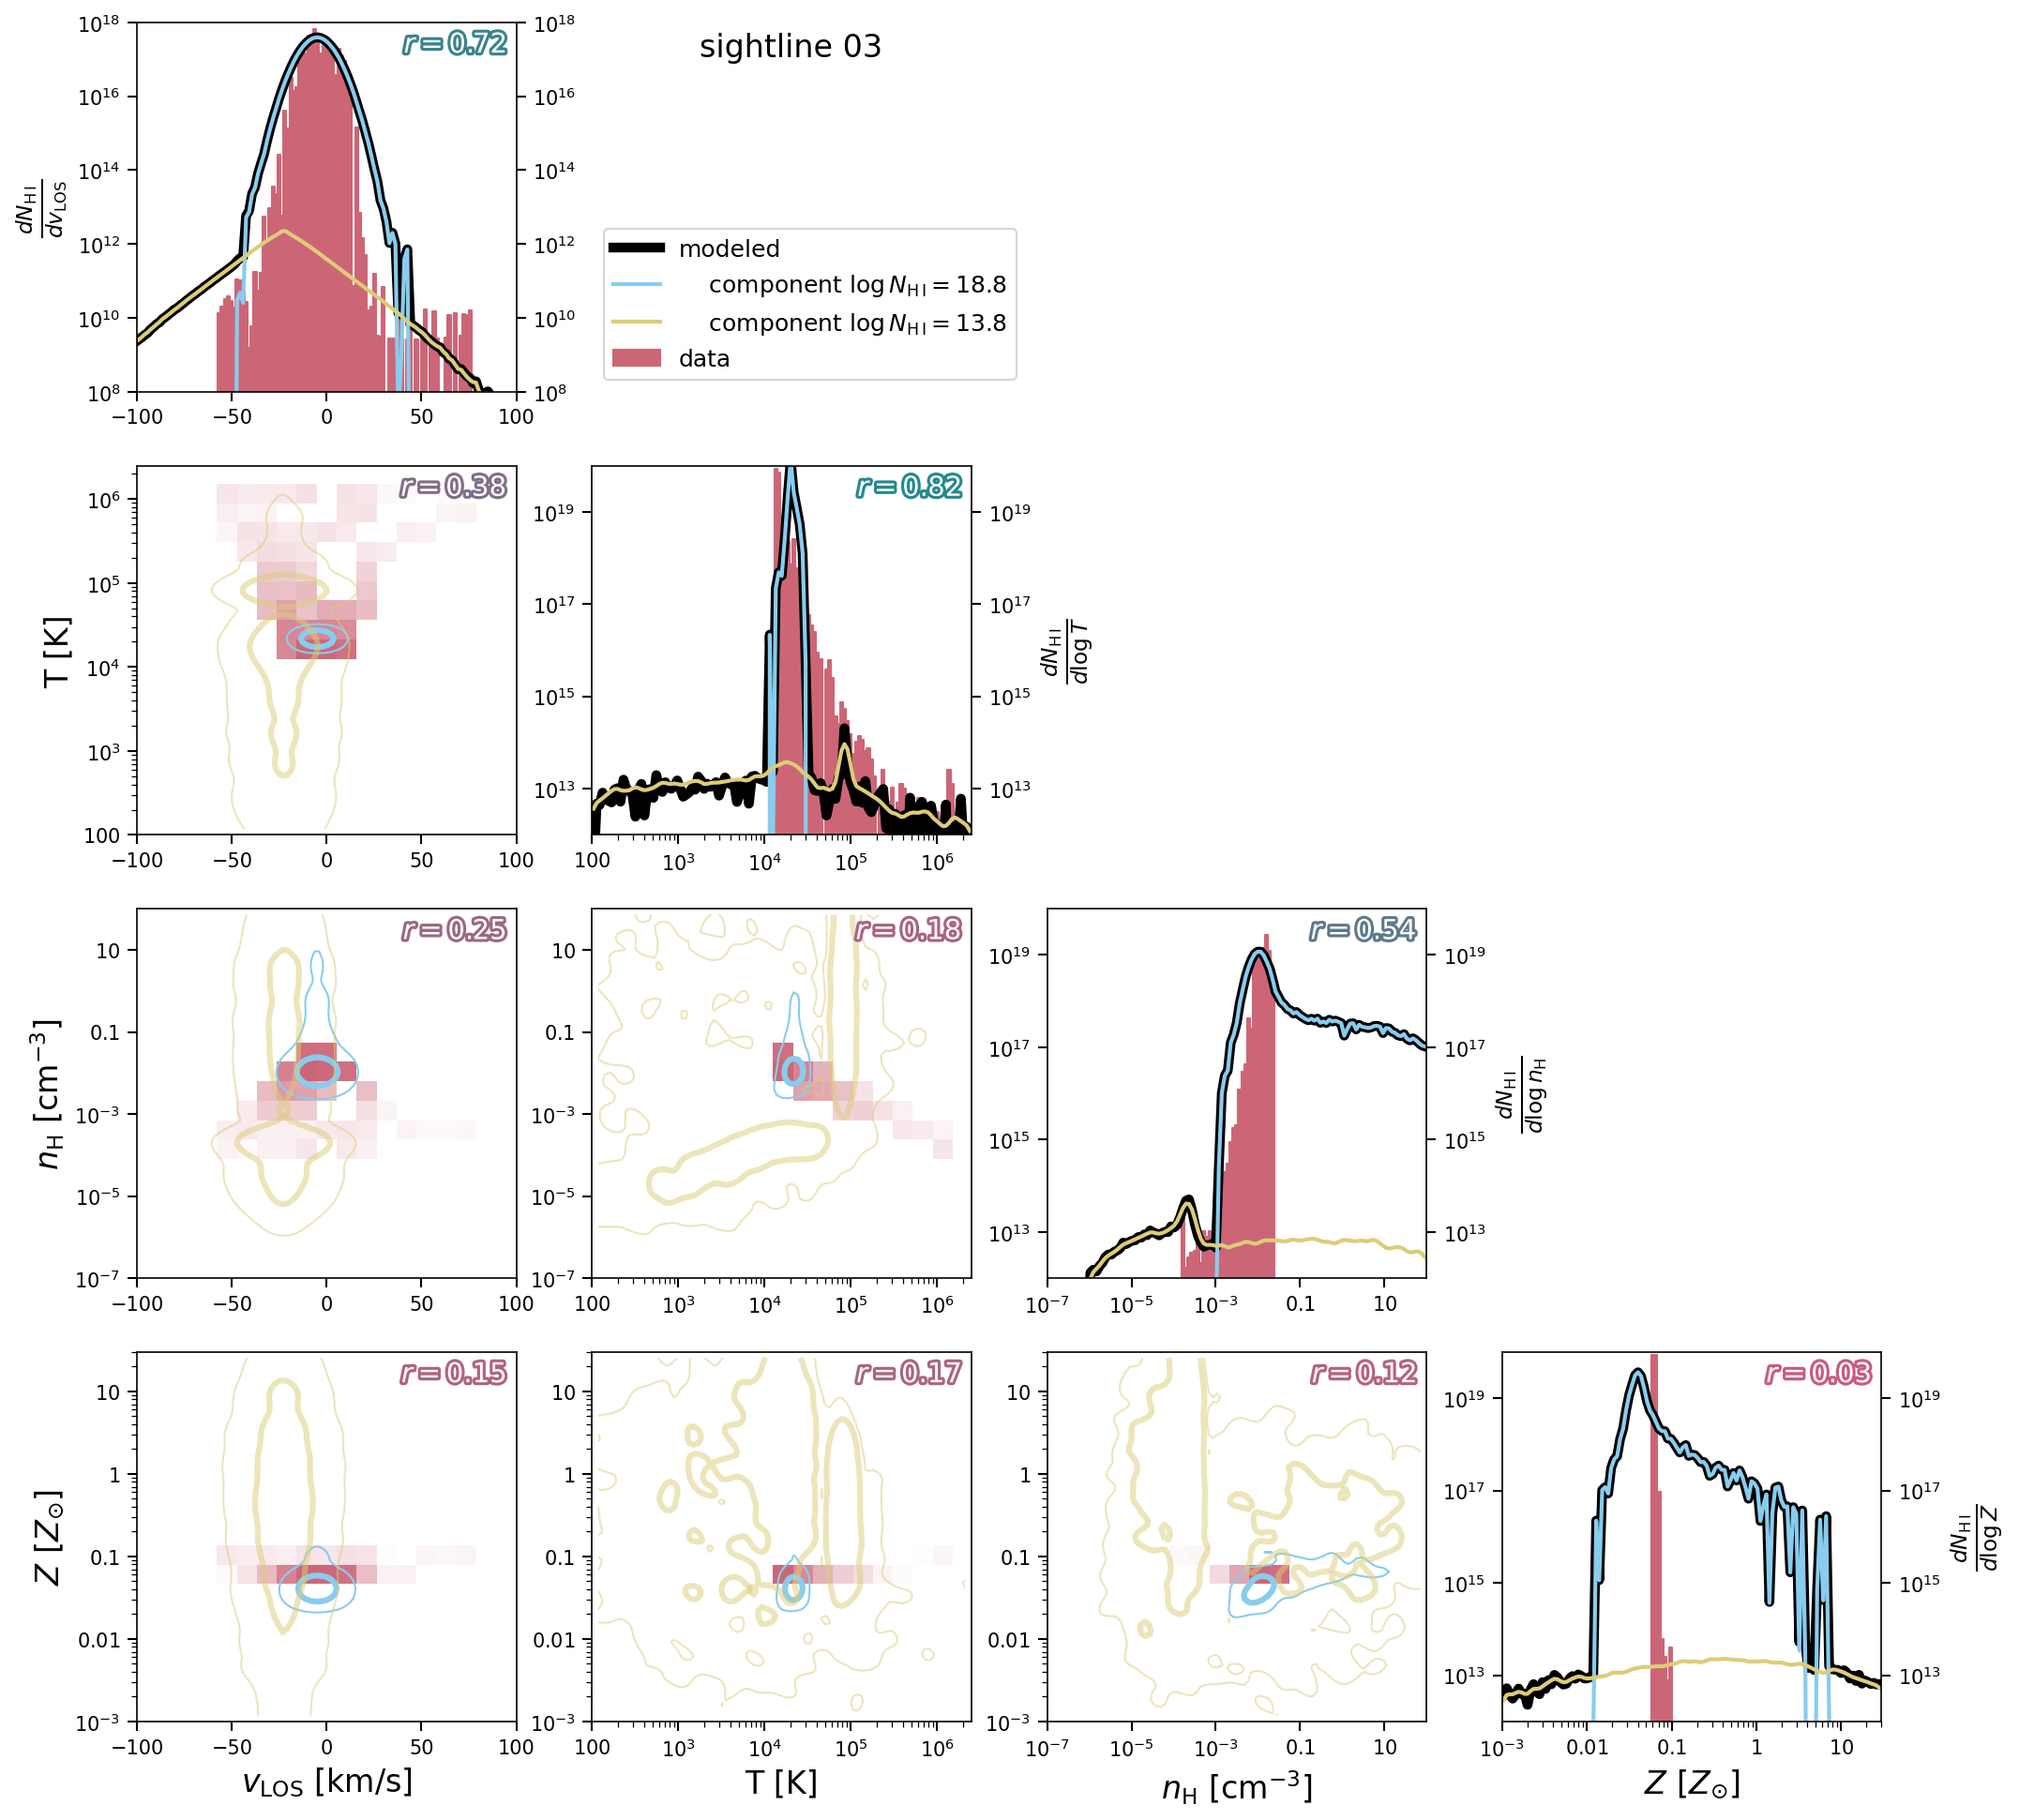
\includegraphics[width=\textwidth]{figures/sample2/sightline_0003.png}
    \label{f: sample2 03}
\end{figure*}

\begin{figure*}
    \centering
    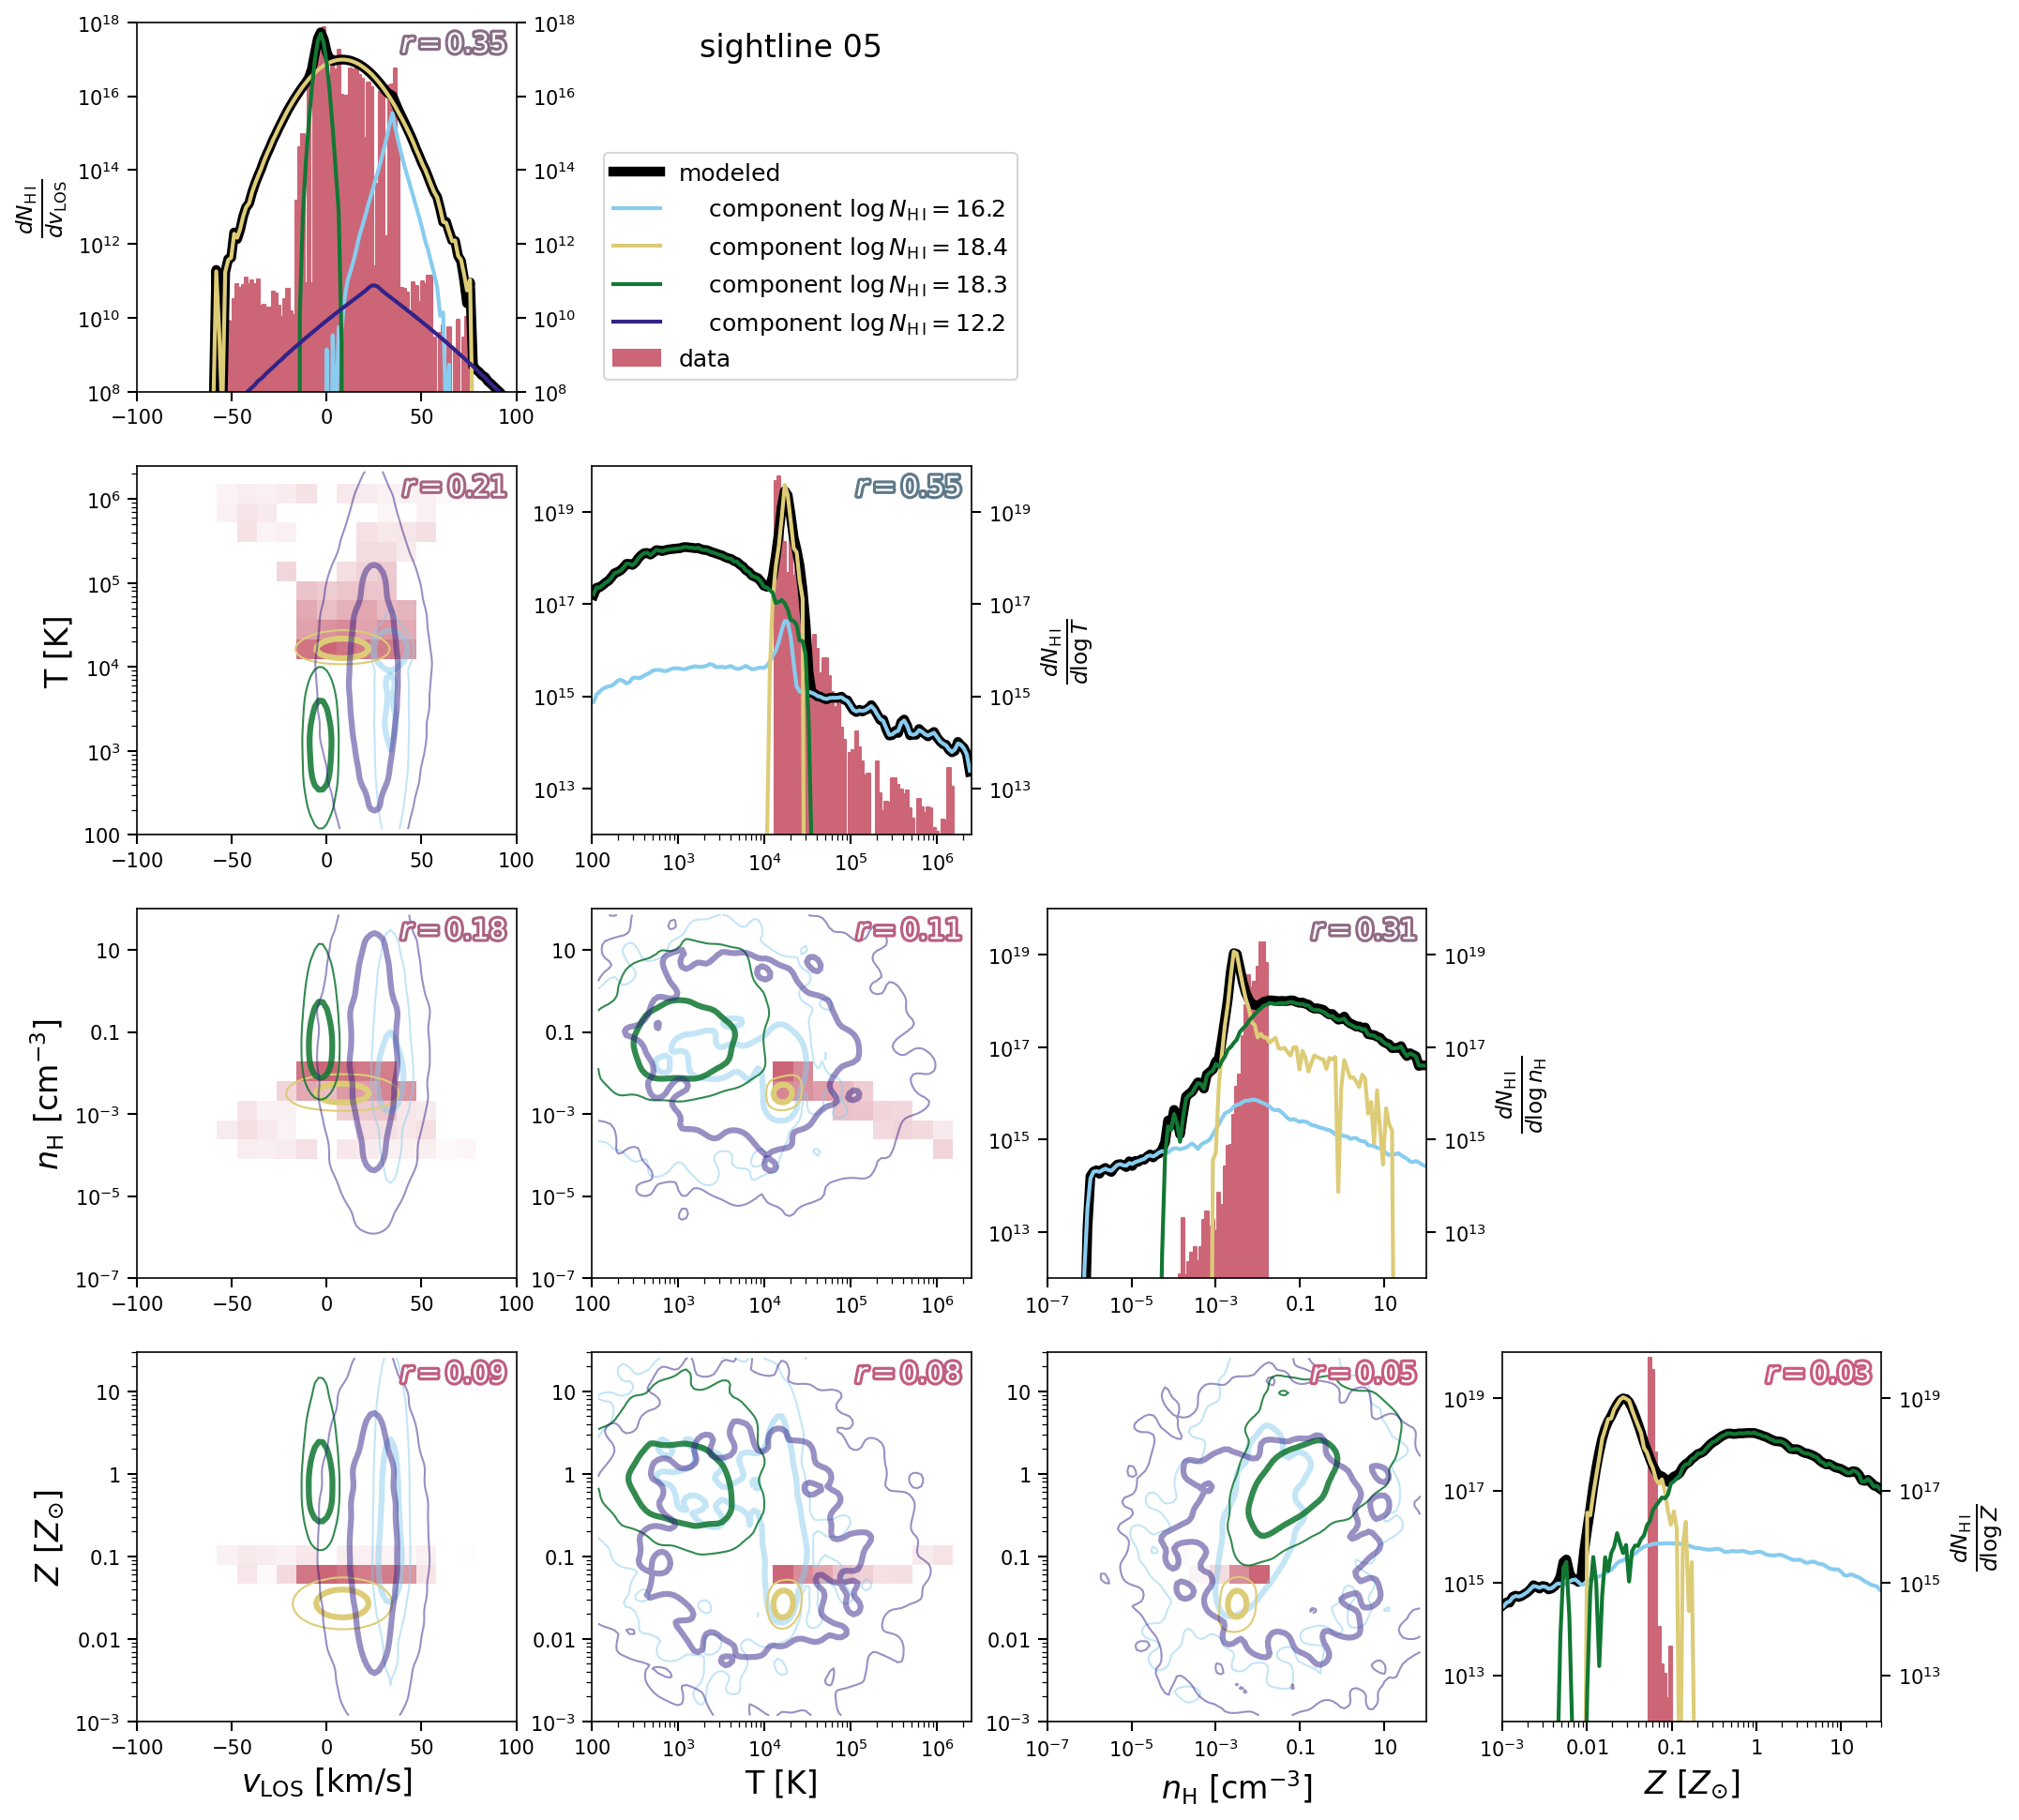
\includegraphics[width=\textwidth]{figures/sample2/sightline_0005.png}
    \label{f: sample2 05}
    \caption{Same as Fig.~\ref{f: sample2 03}, but for sightline 05.}
\end{figure*}

\begin{figure*}
    \centering
    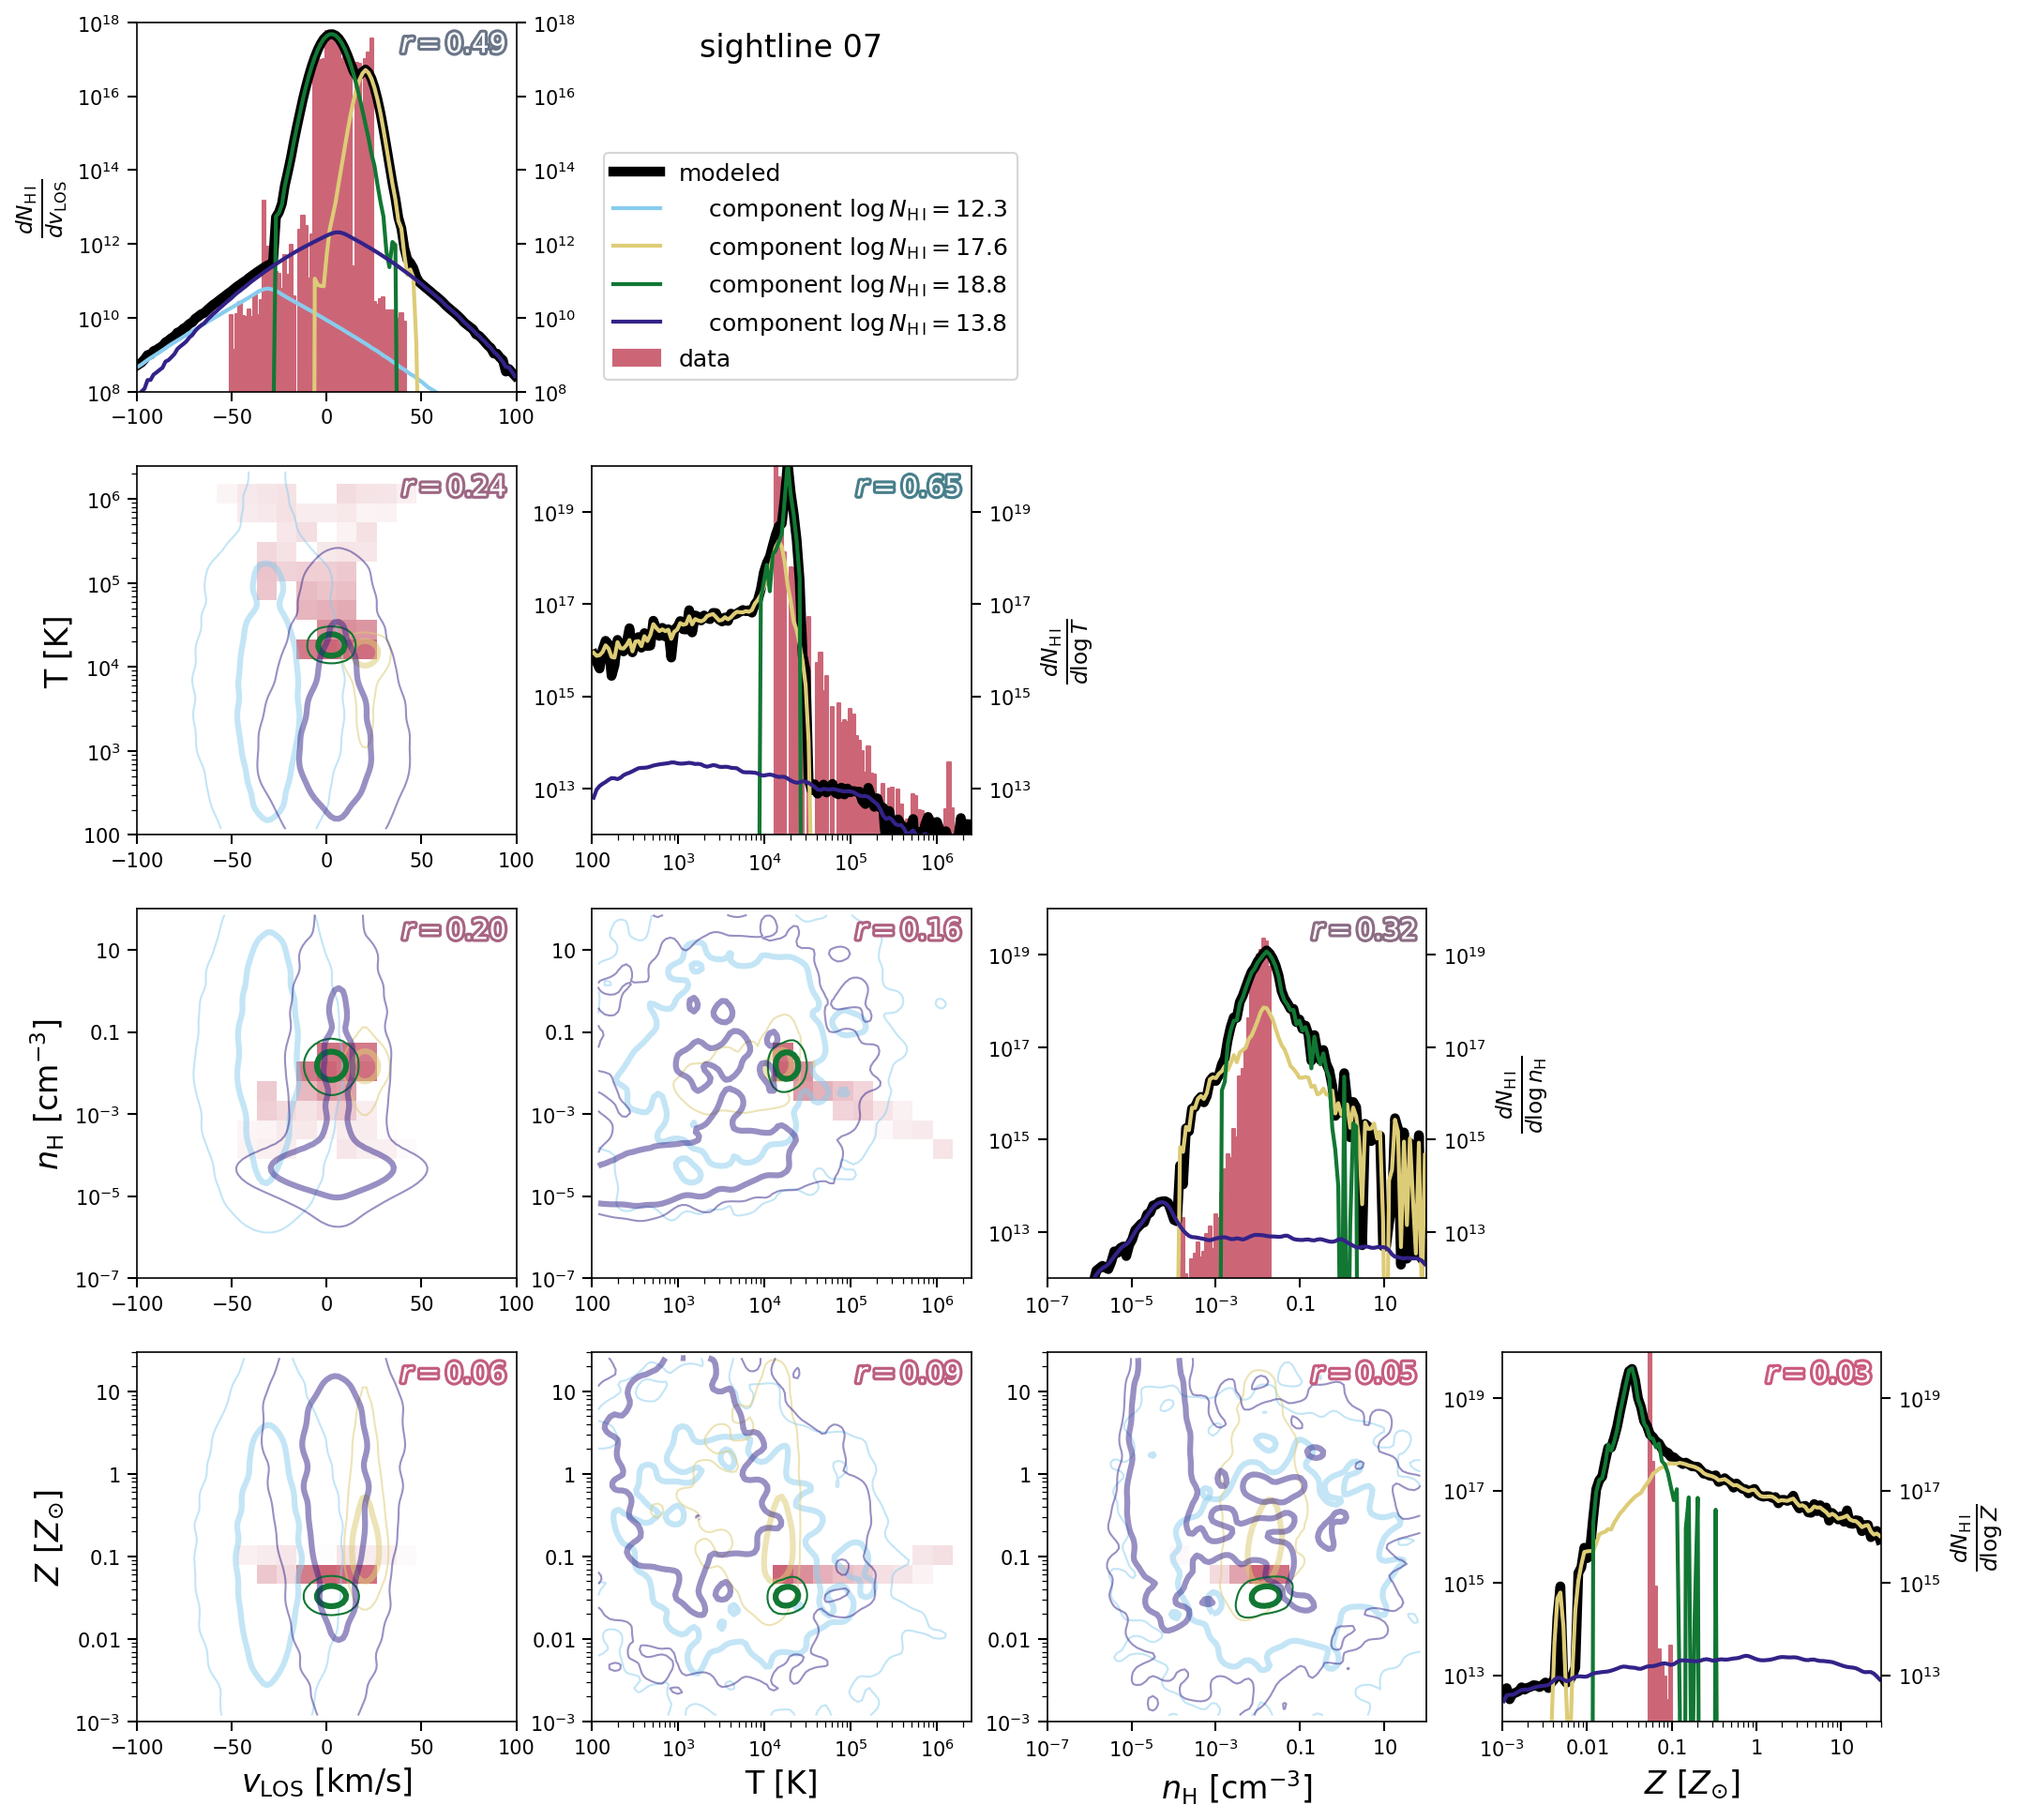
\includegraphics[width=\textwidth]{figures/sample2/sightline_0007.png}
    \label{f: sample2 07}
    \caption{Same as Fig.~\ref{f: sample2 03}, but for sightline 07.}
\end{figure*}

\begin{figure*}
    \centering
    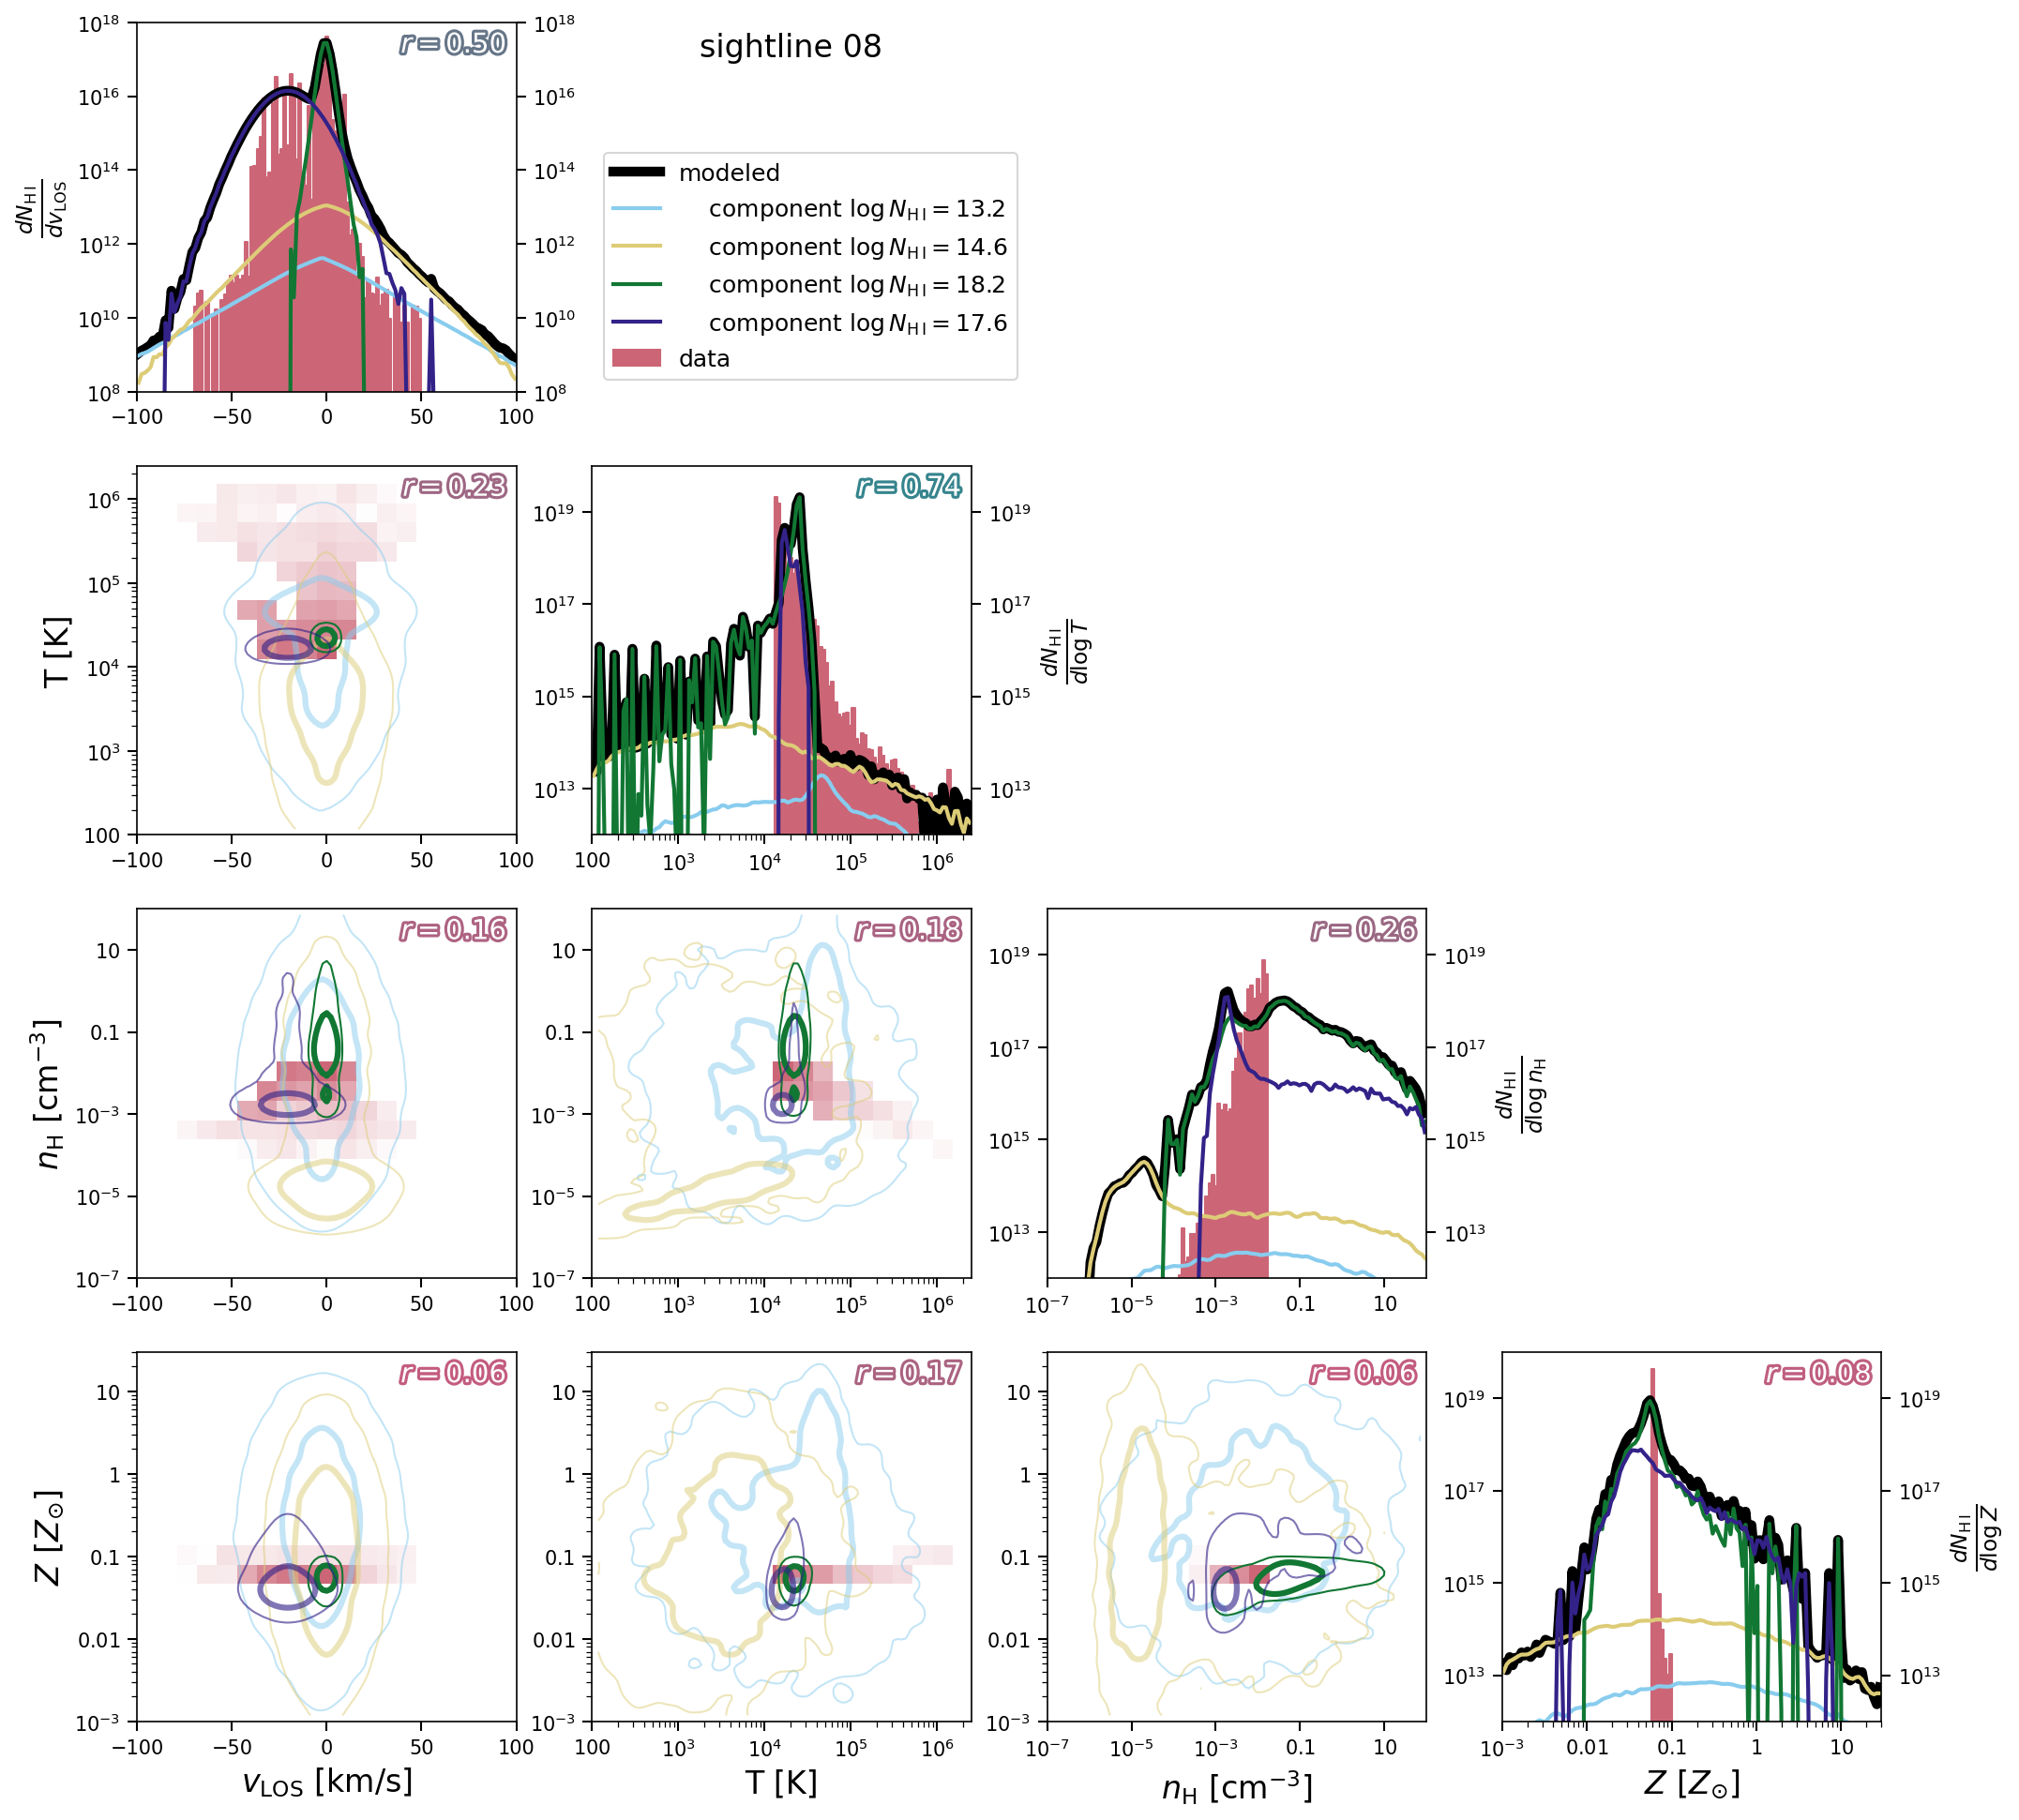
\includegraphics[width=\textwidth]{figures/sample2/sightline_0008.png}
    \label{f: sample2 08}
    \caption{Same as Fig.~\ref{f: sample2 03}, but for sightline 08.}
\end{figure*}

\begin{figure*}
    \centering
    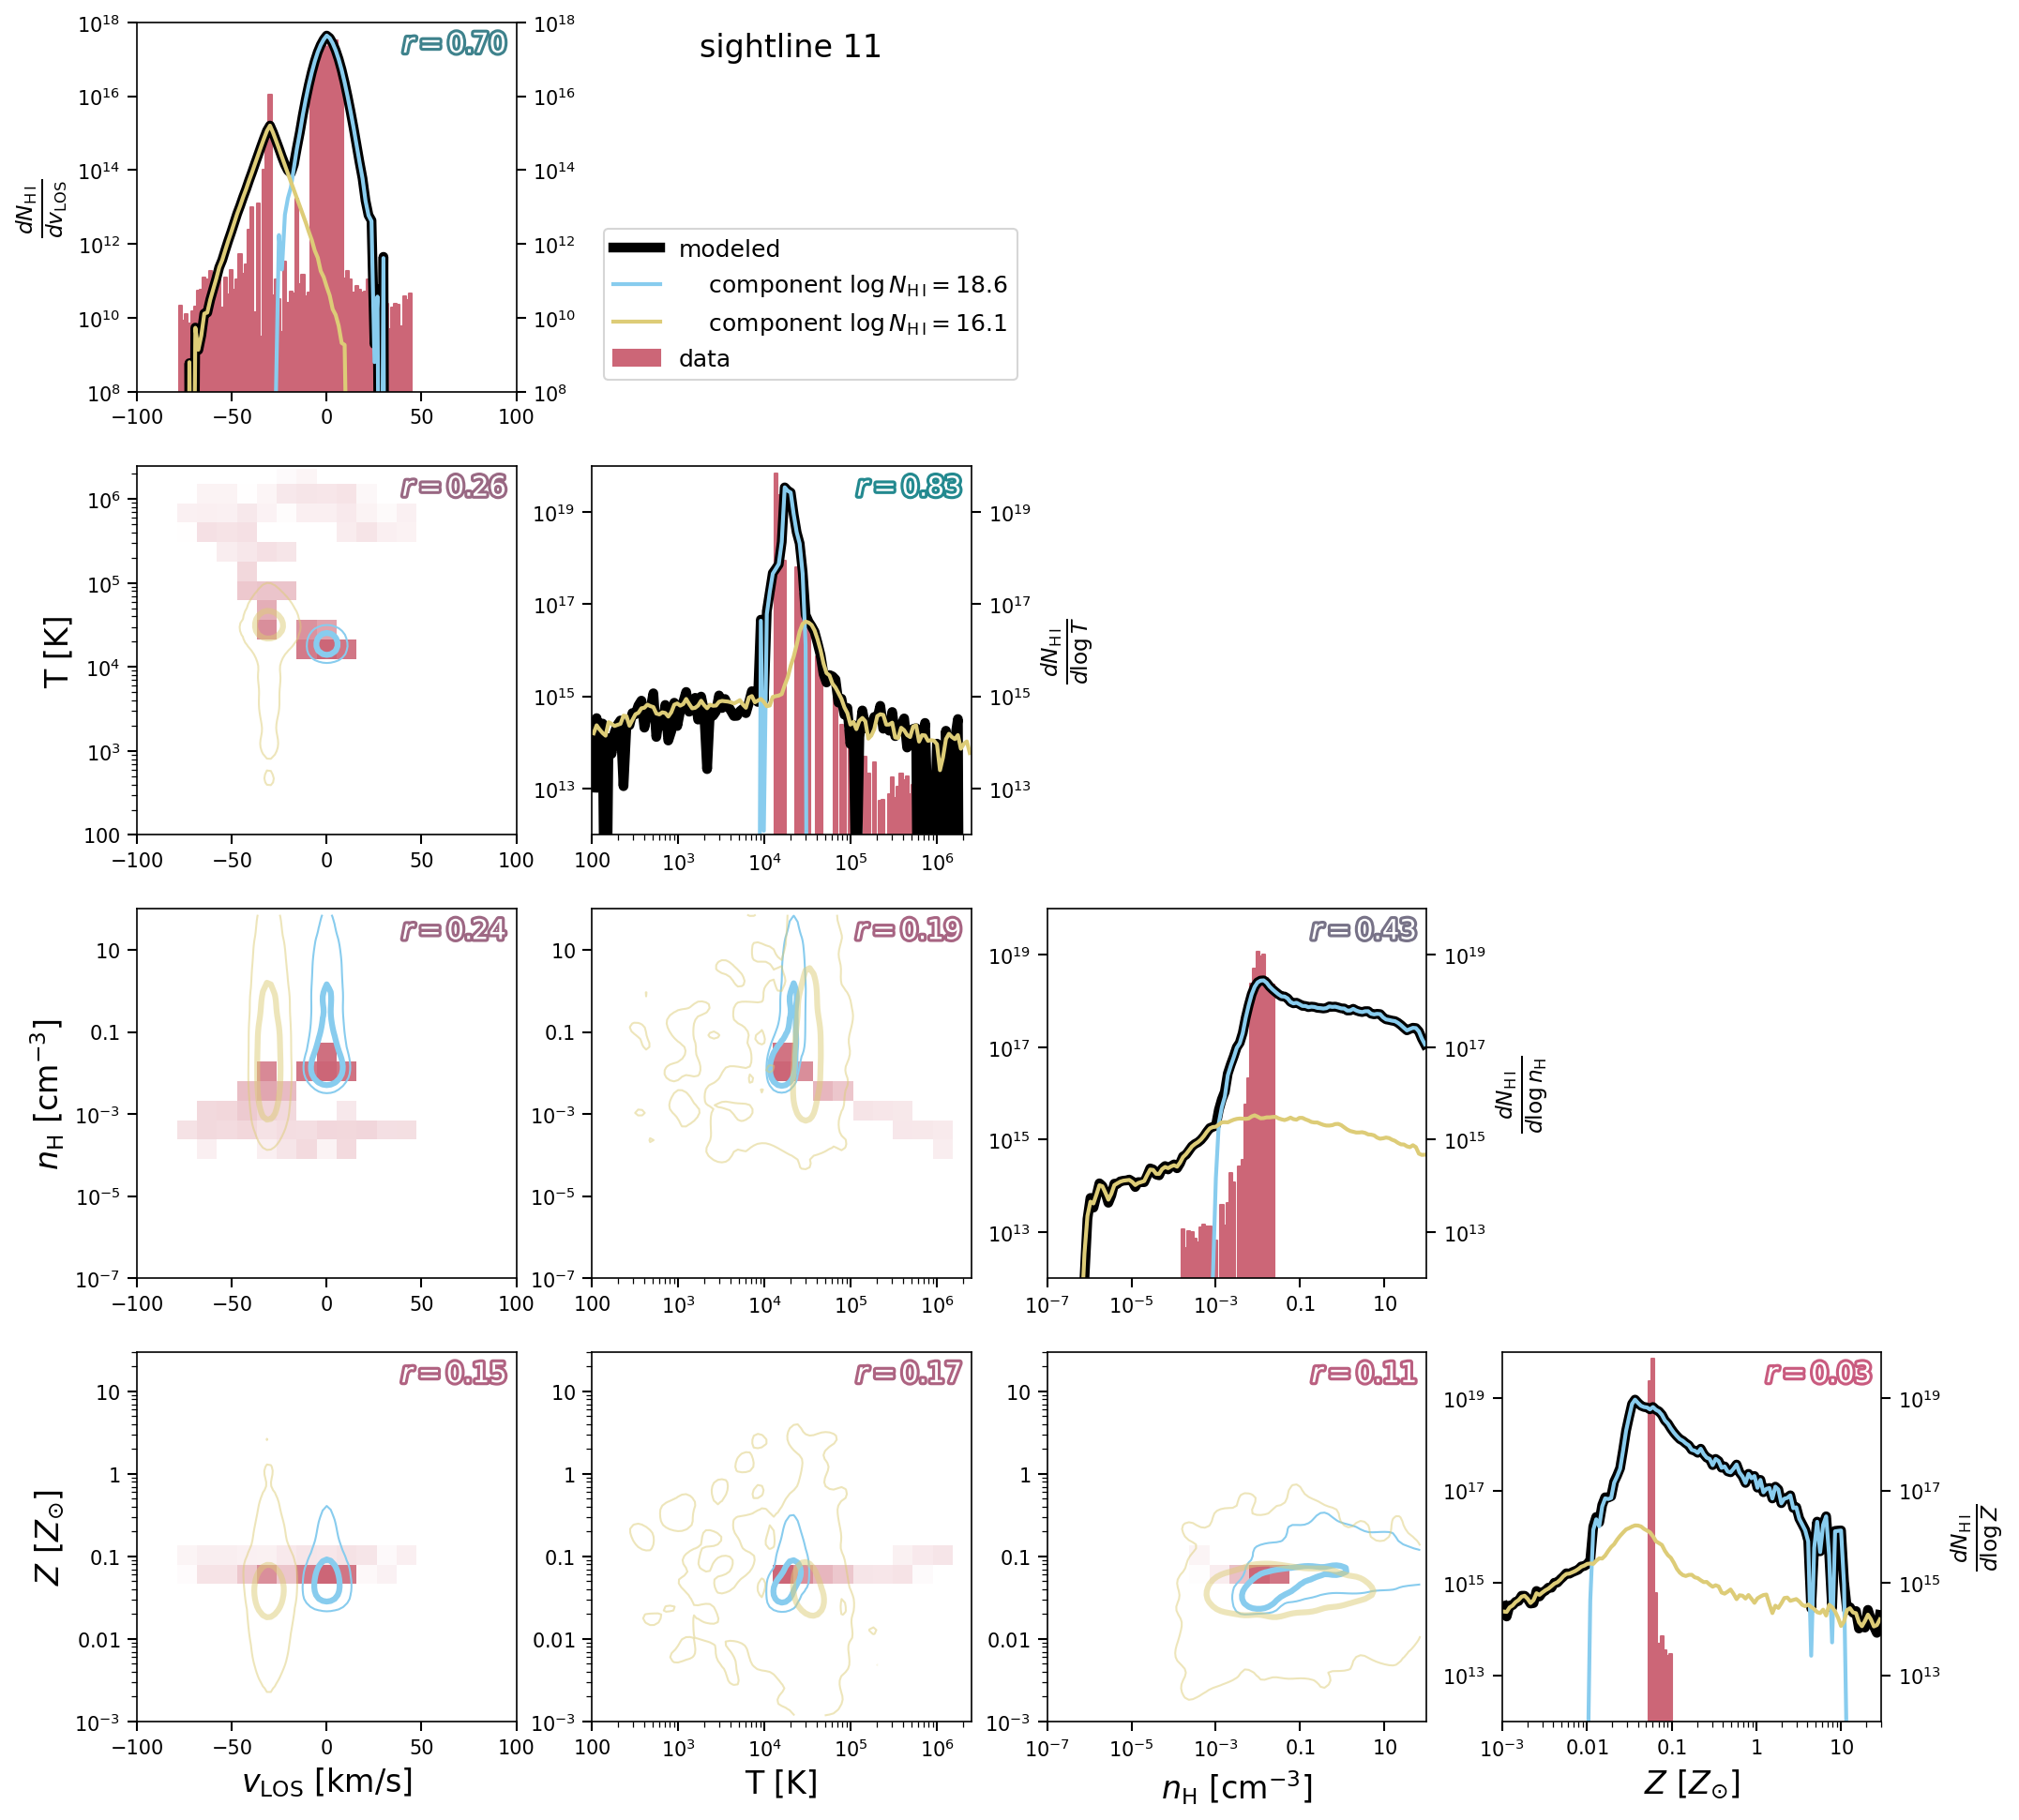
\includegraphics[width=\textwidth]{figures/sample2/sightline_0011.png}
    \label{f: sample2 11}
    \caption{Same as Fig.~\ref{f: sample2 03}, but for sightline 11.}
\end{figure*}

\begin{figure*}
    \centering
    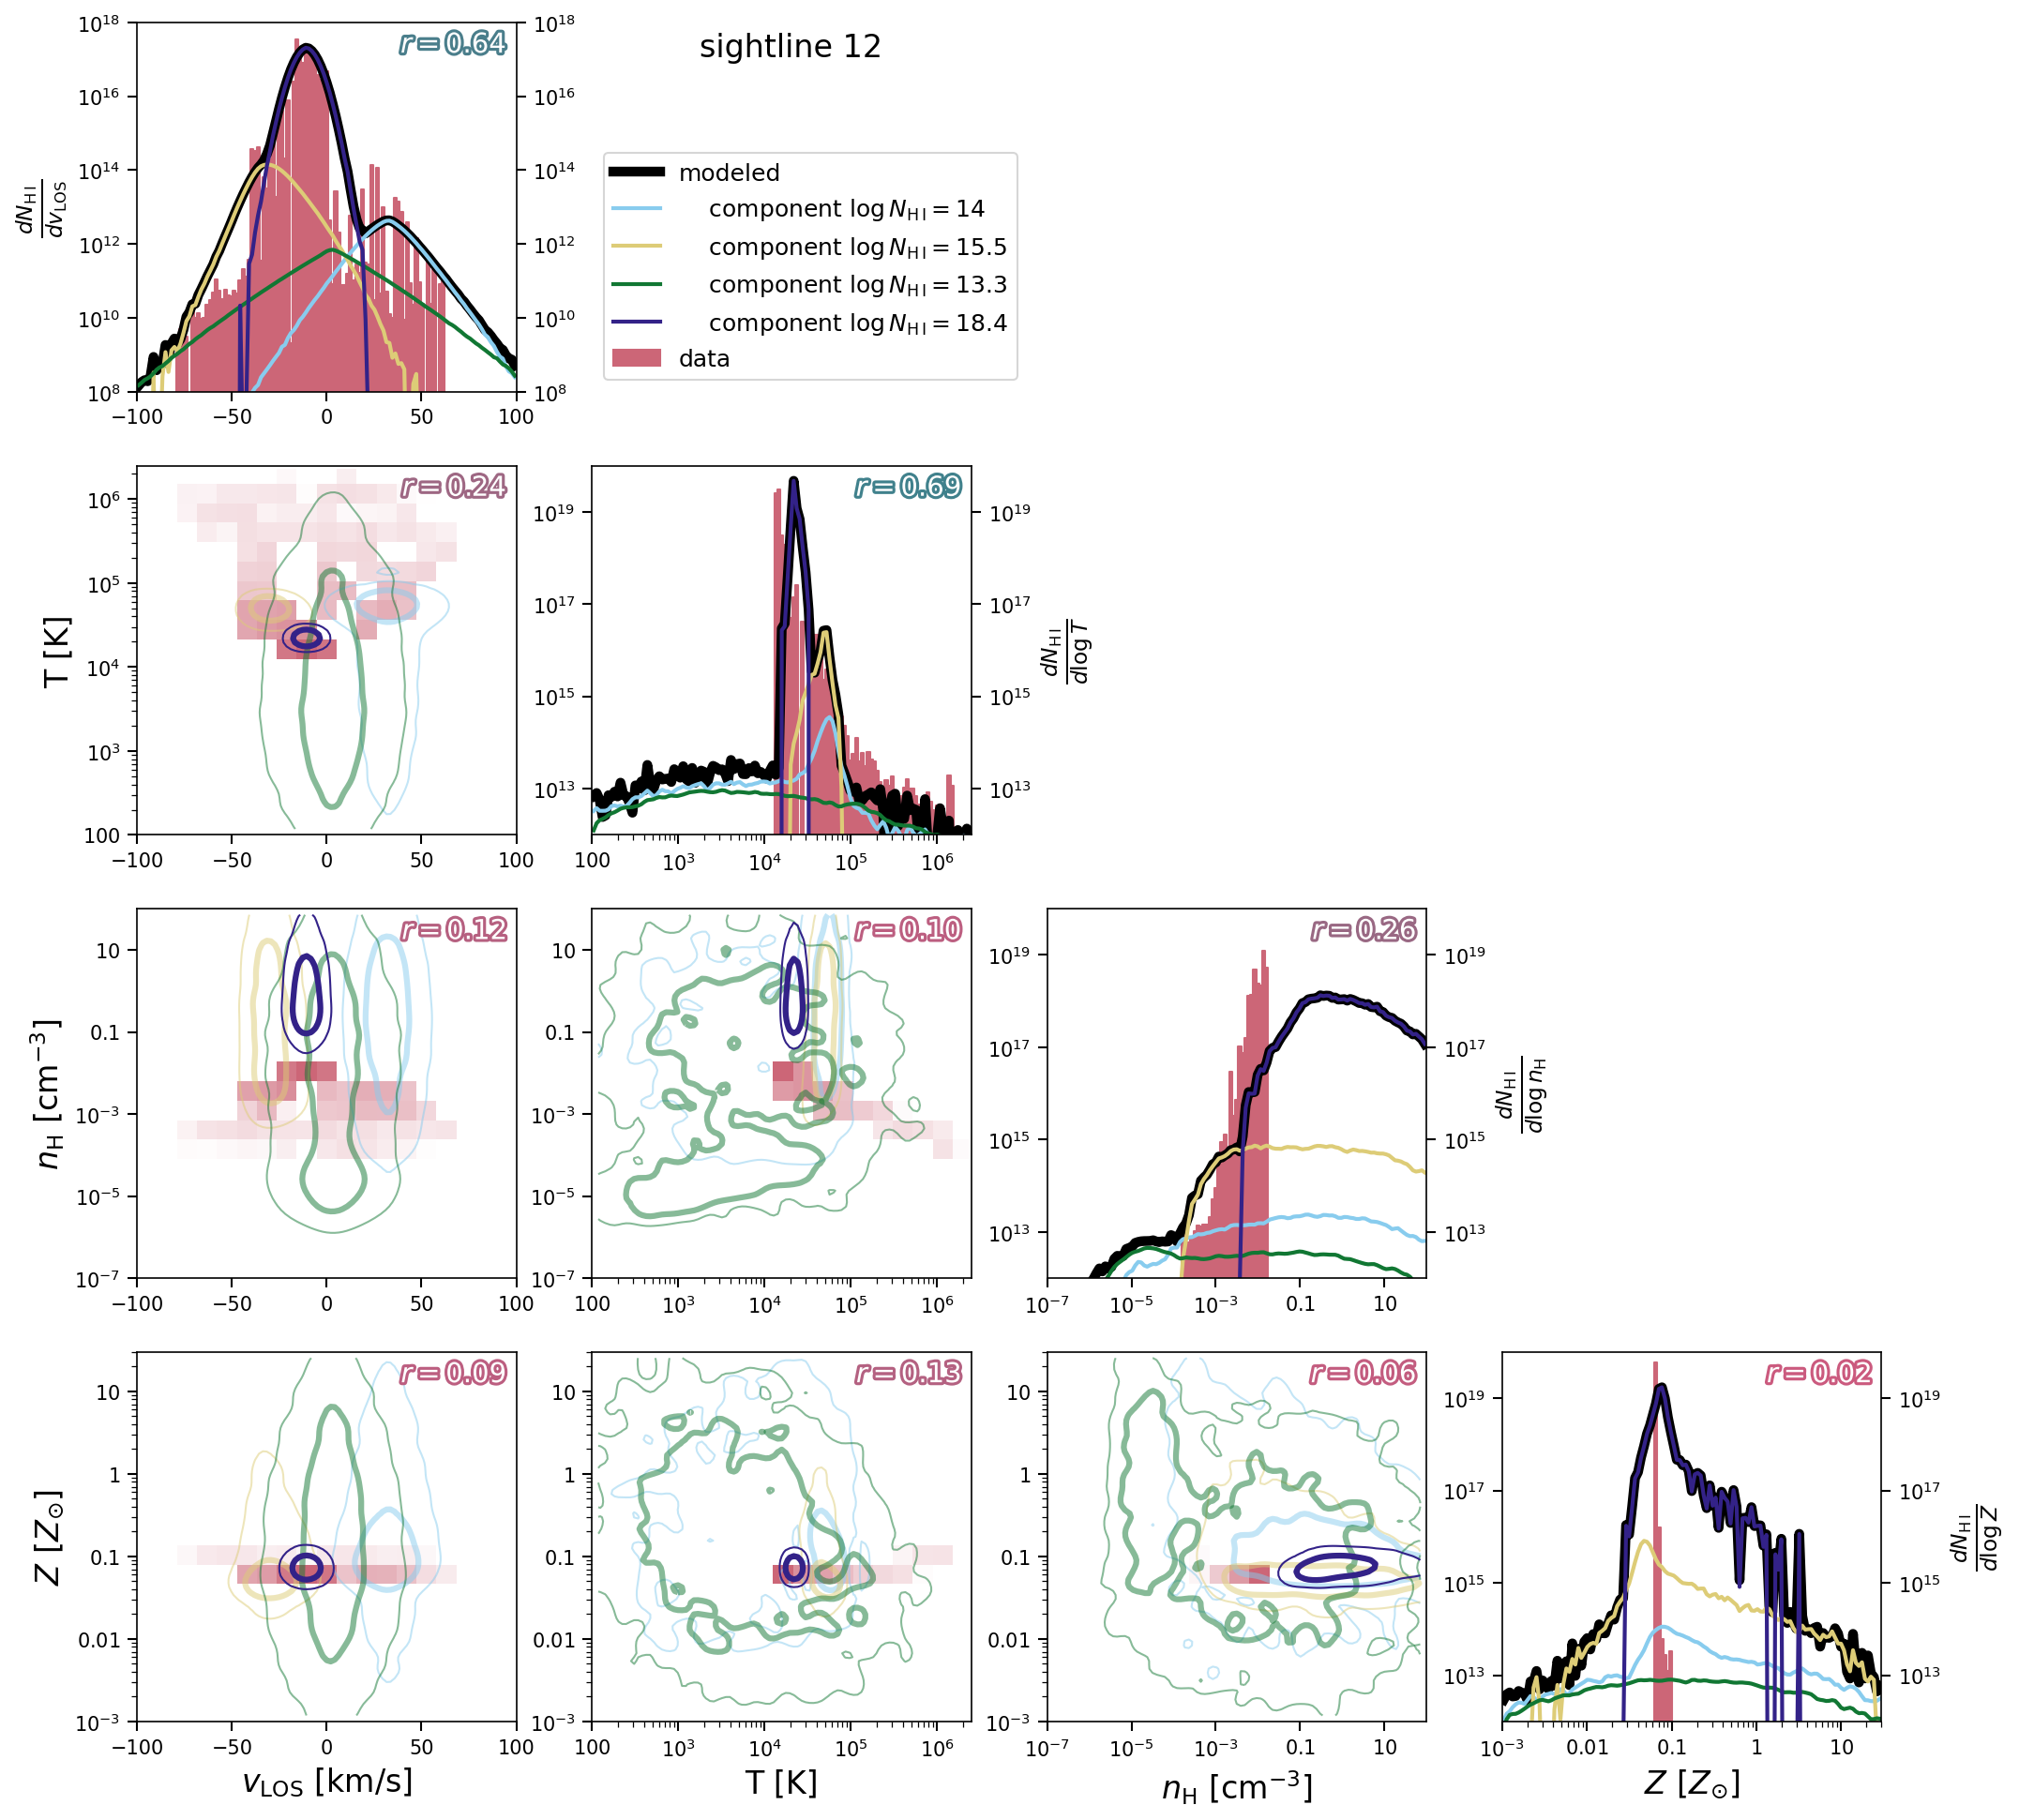
\includegraphics[width=\textwidth]{figures/sample2/sightline_0012.png}
    \label{f: sample2 12}
    \caption{Same as Fig.~\ref{f: sample2 03}, but for sightline 12.}
\end{figure*}

\begin{figure*}
    \centering
    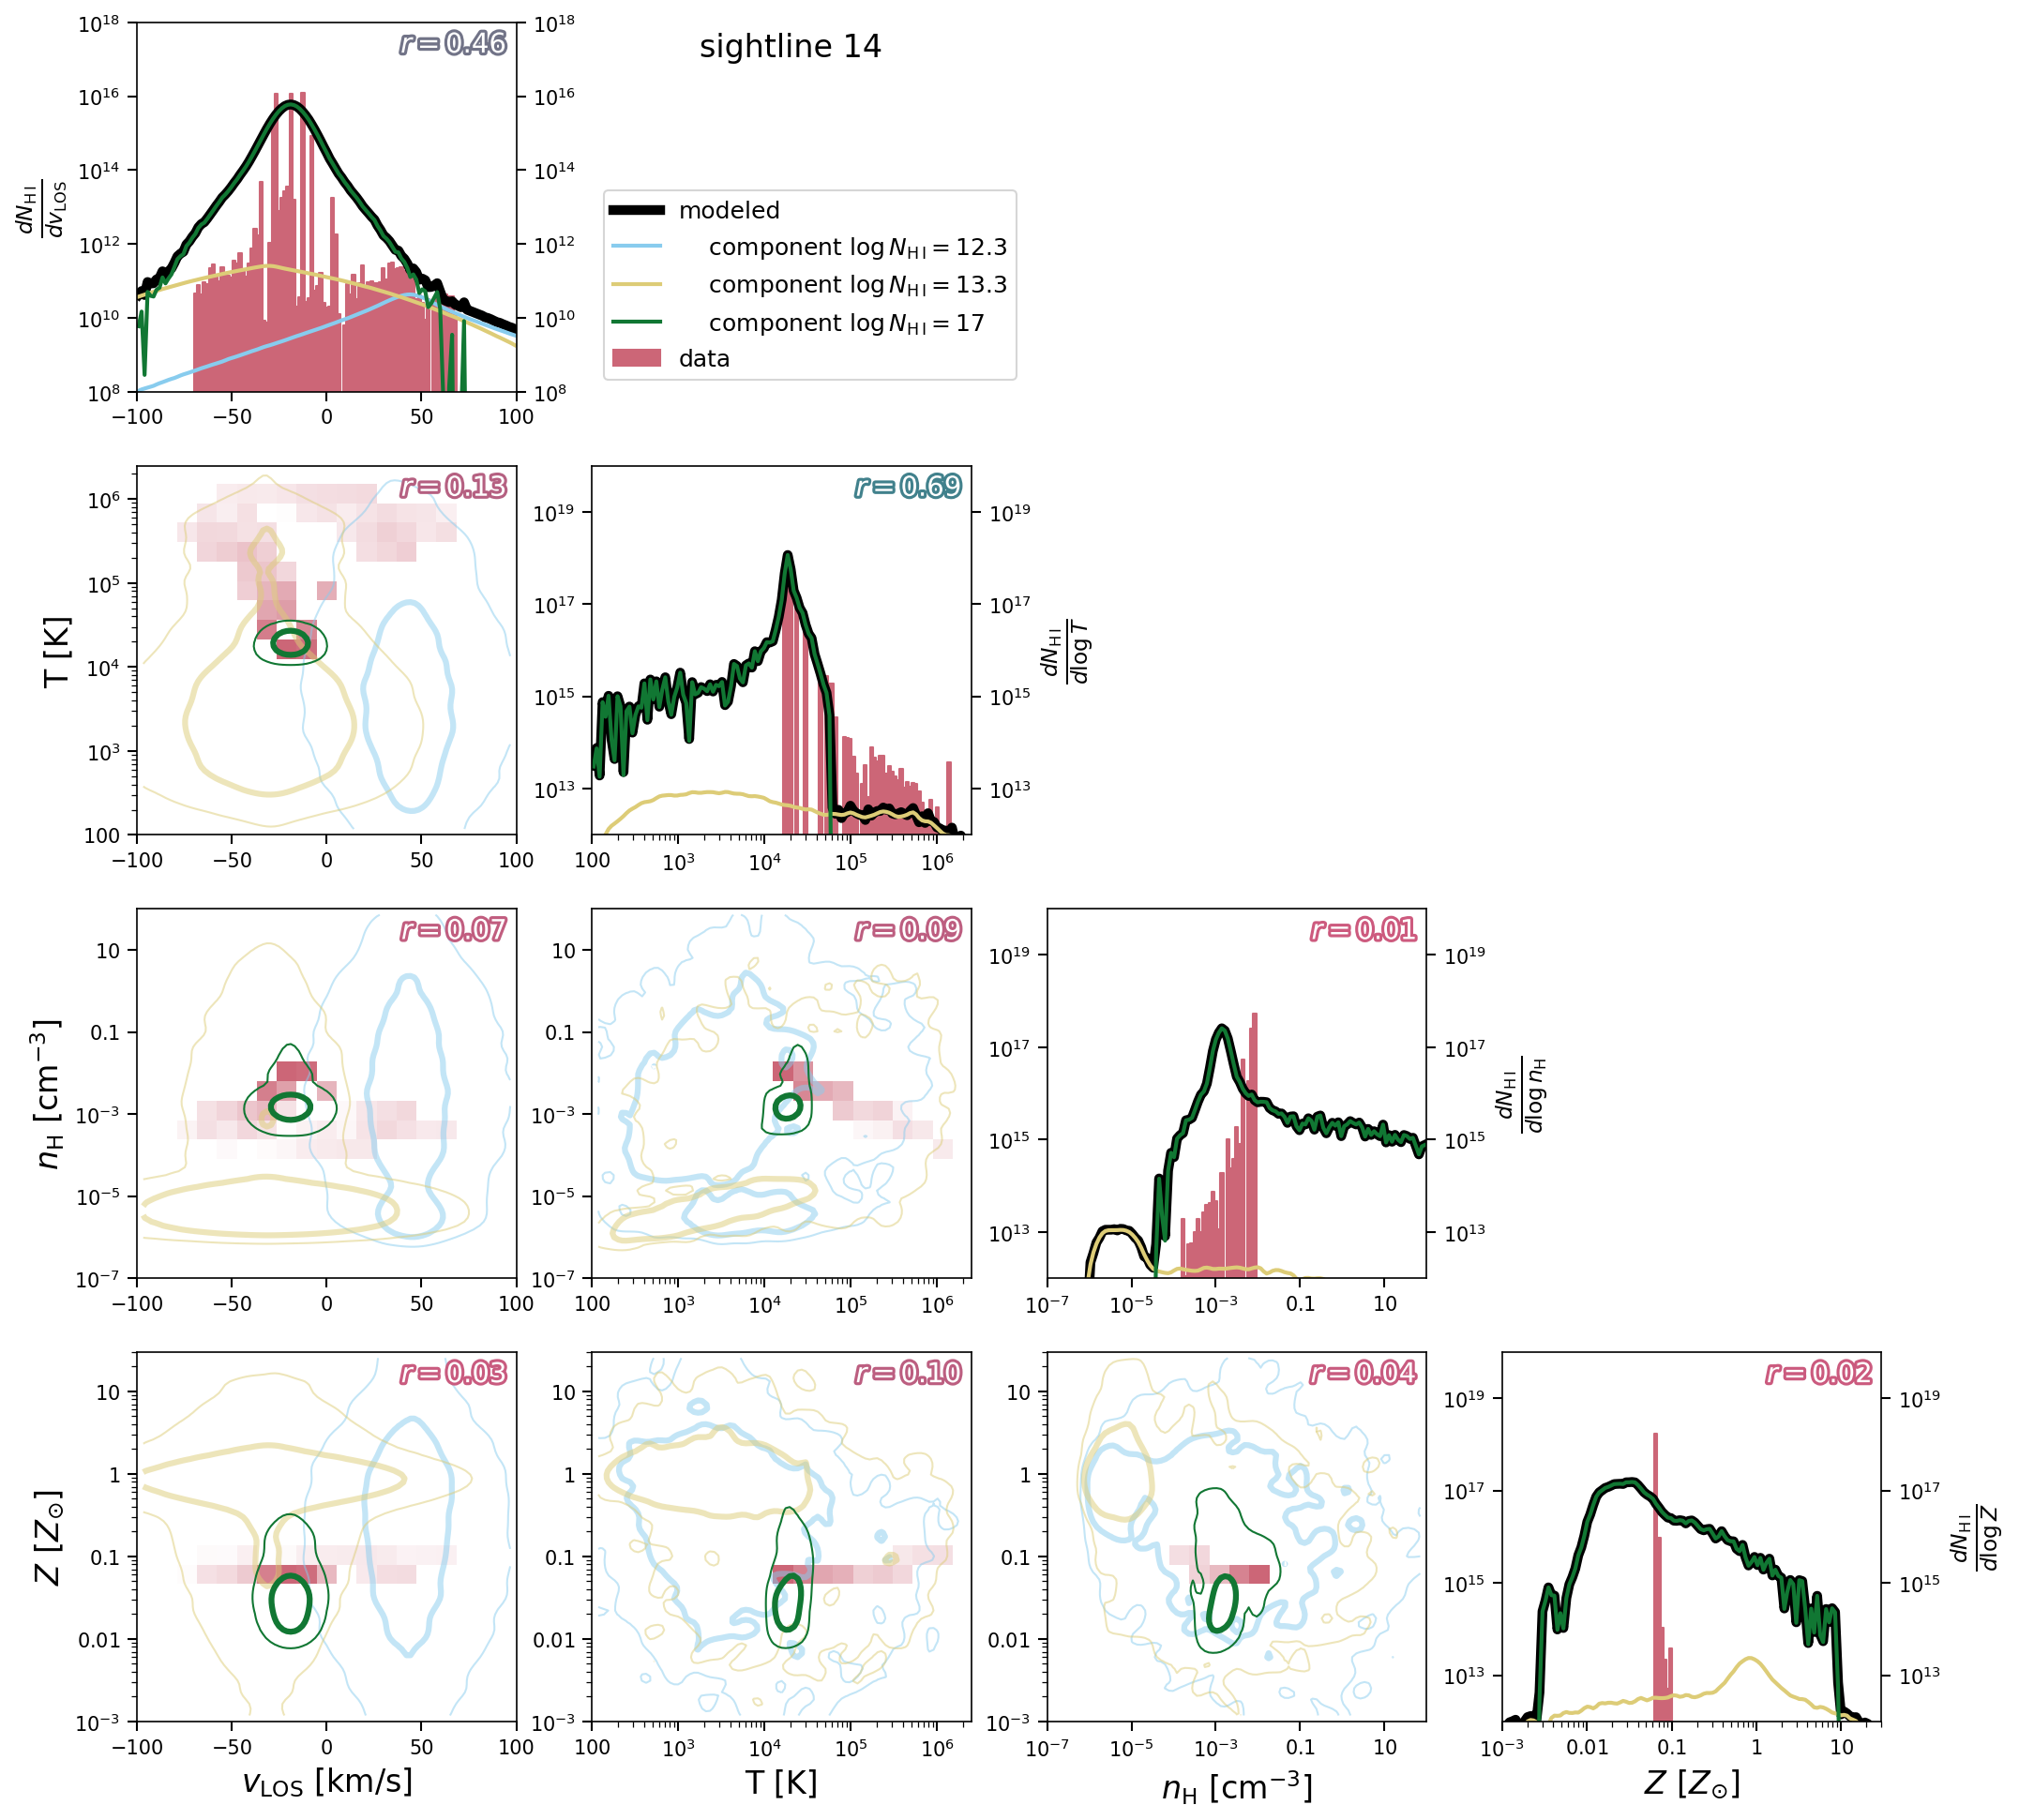
\includegraphics[width=\textwidth]{figures/sample2/sightline_0014.png}
    \label{f: sample2 14}
    \caption{Same as Fig.~\ref{f: sample2 03}, but for sightline 14.}
\end{figure*}

\begin{figure*}
    \centering
    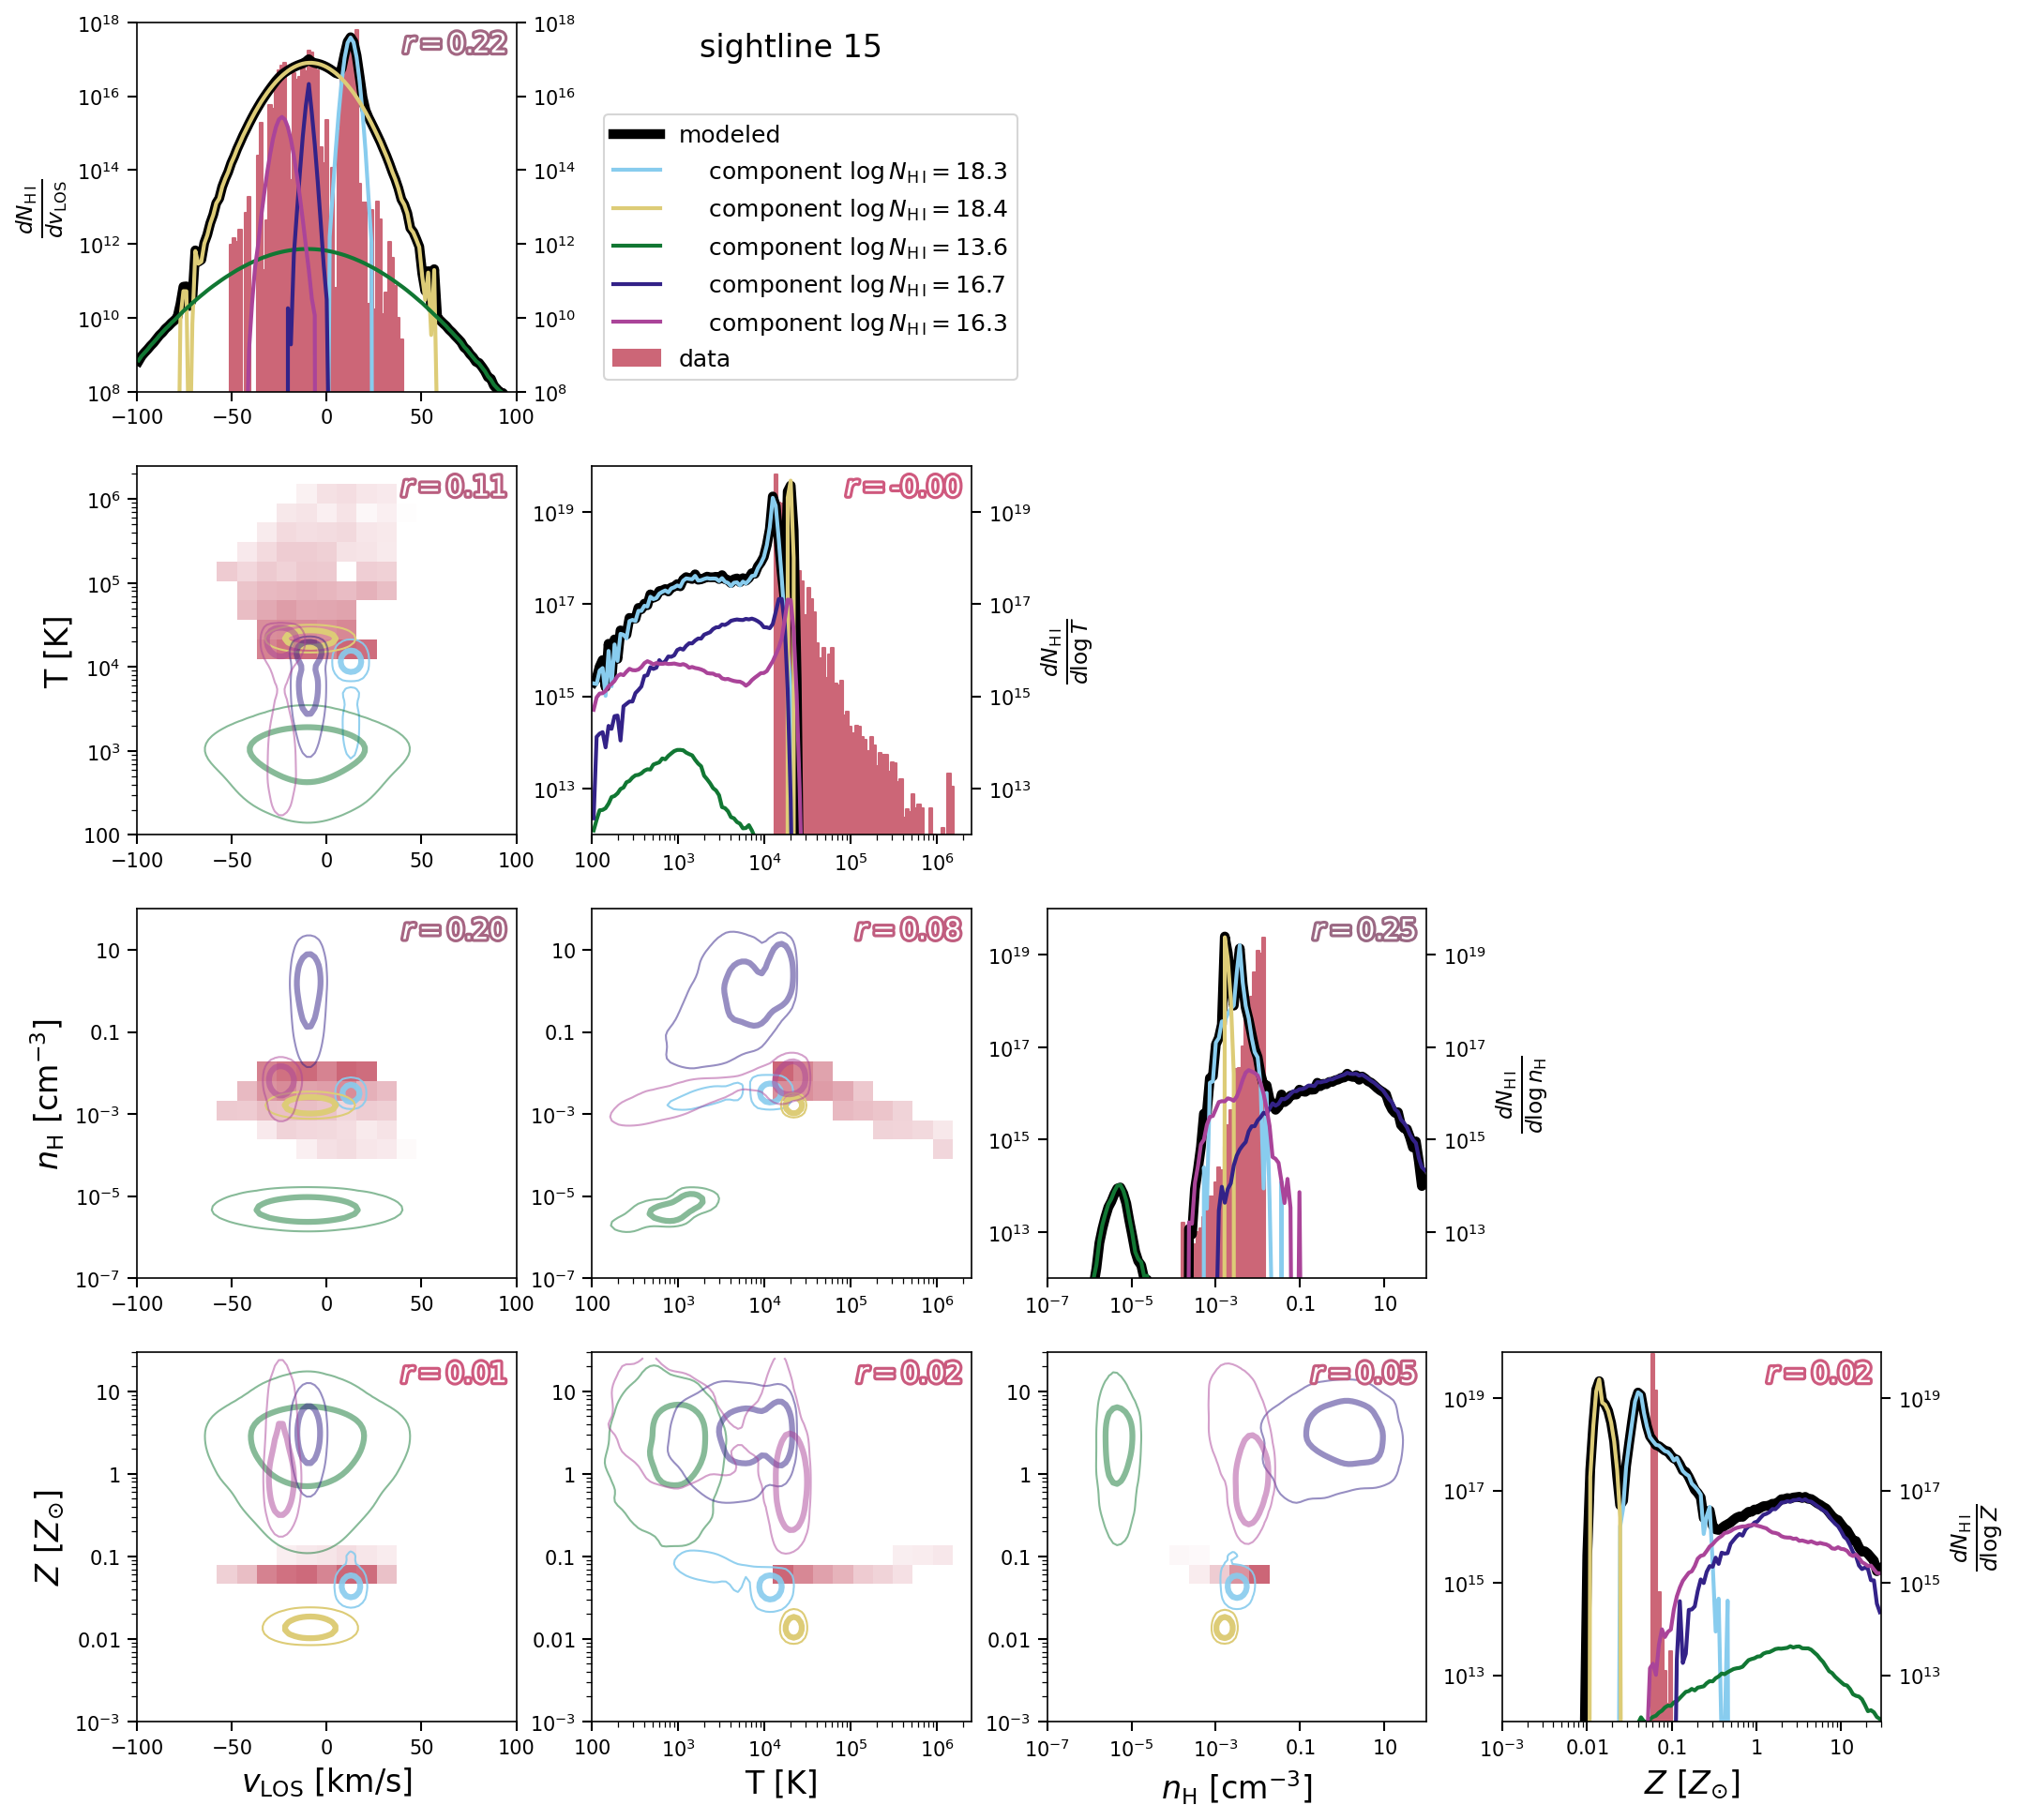
\includegraphics[width=\textwidth]{figures/sample2/sightline_0015.png}
    \label{f: sample2 15}
    \caption{Same as Fig.~\ref{f: sample2 03}, but for sightline 15.}
\end{figure*}

\begin{figure*}
    \centering
    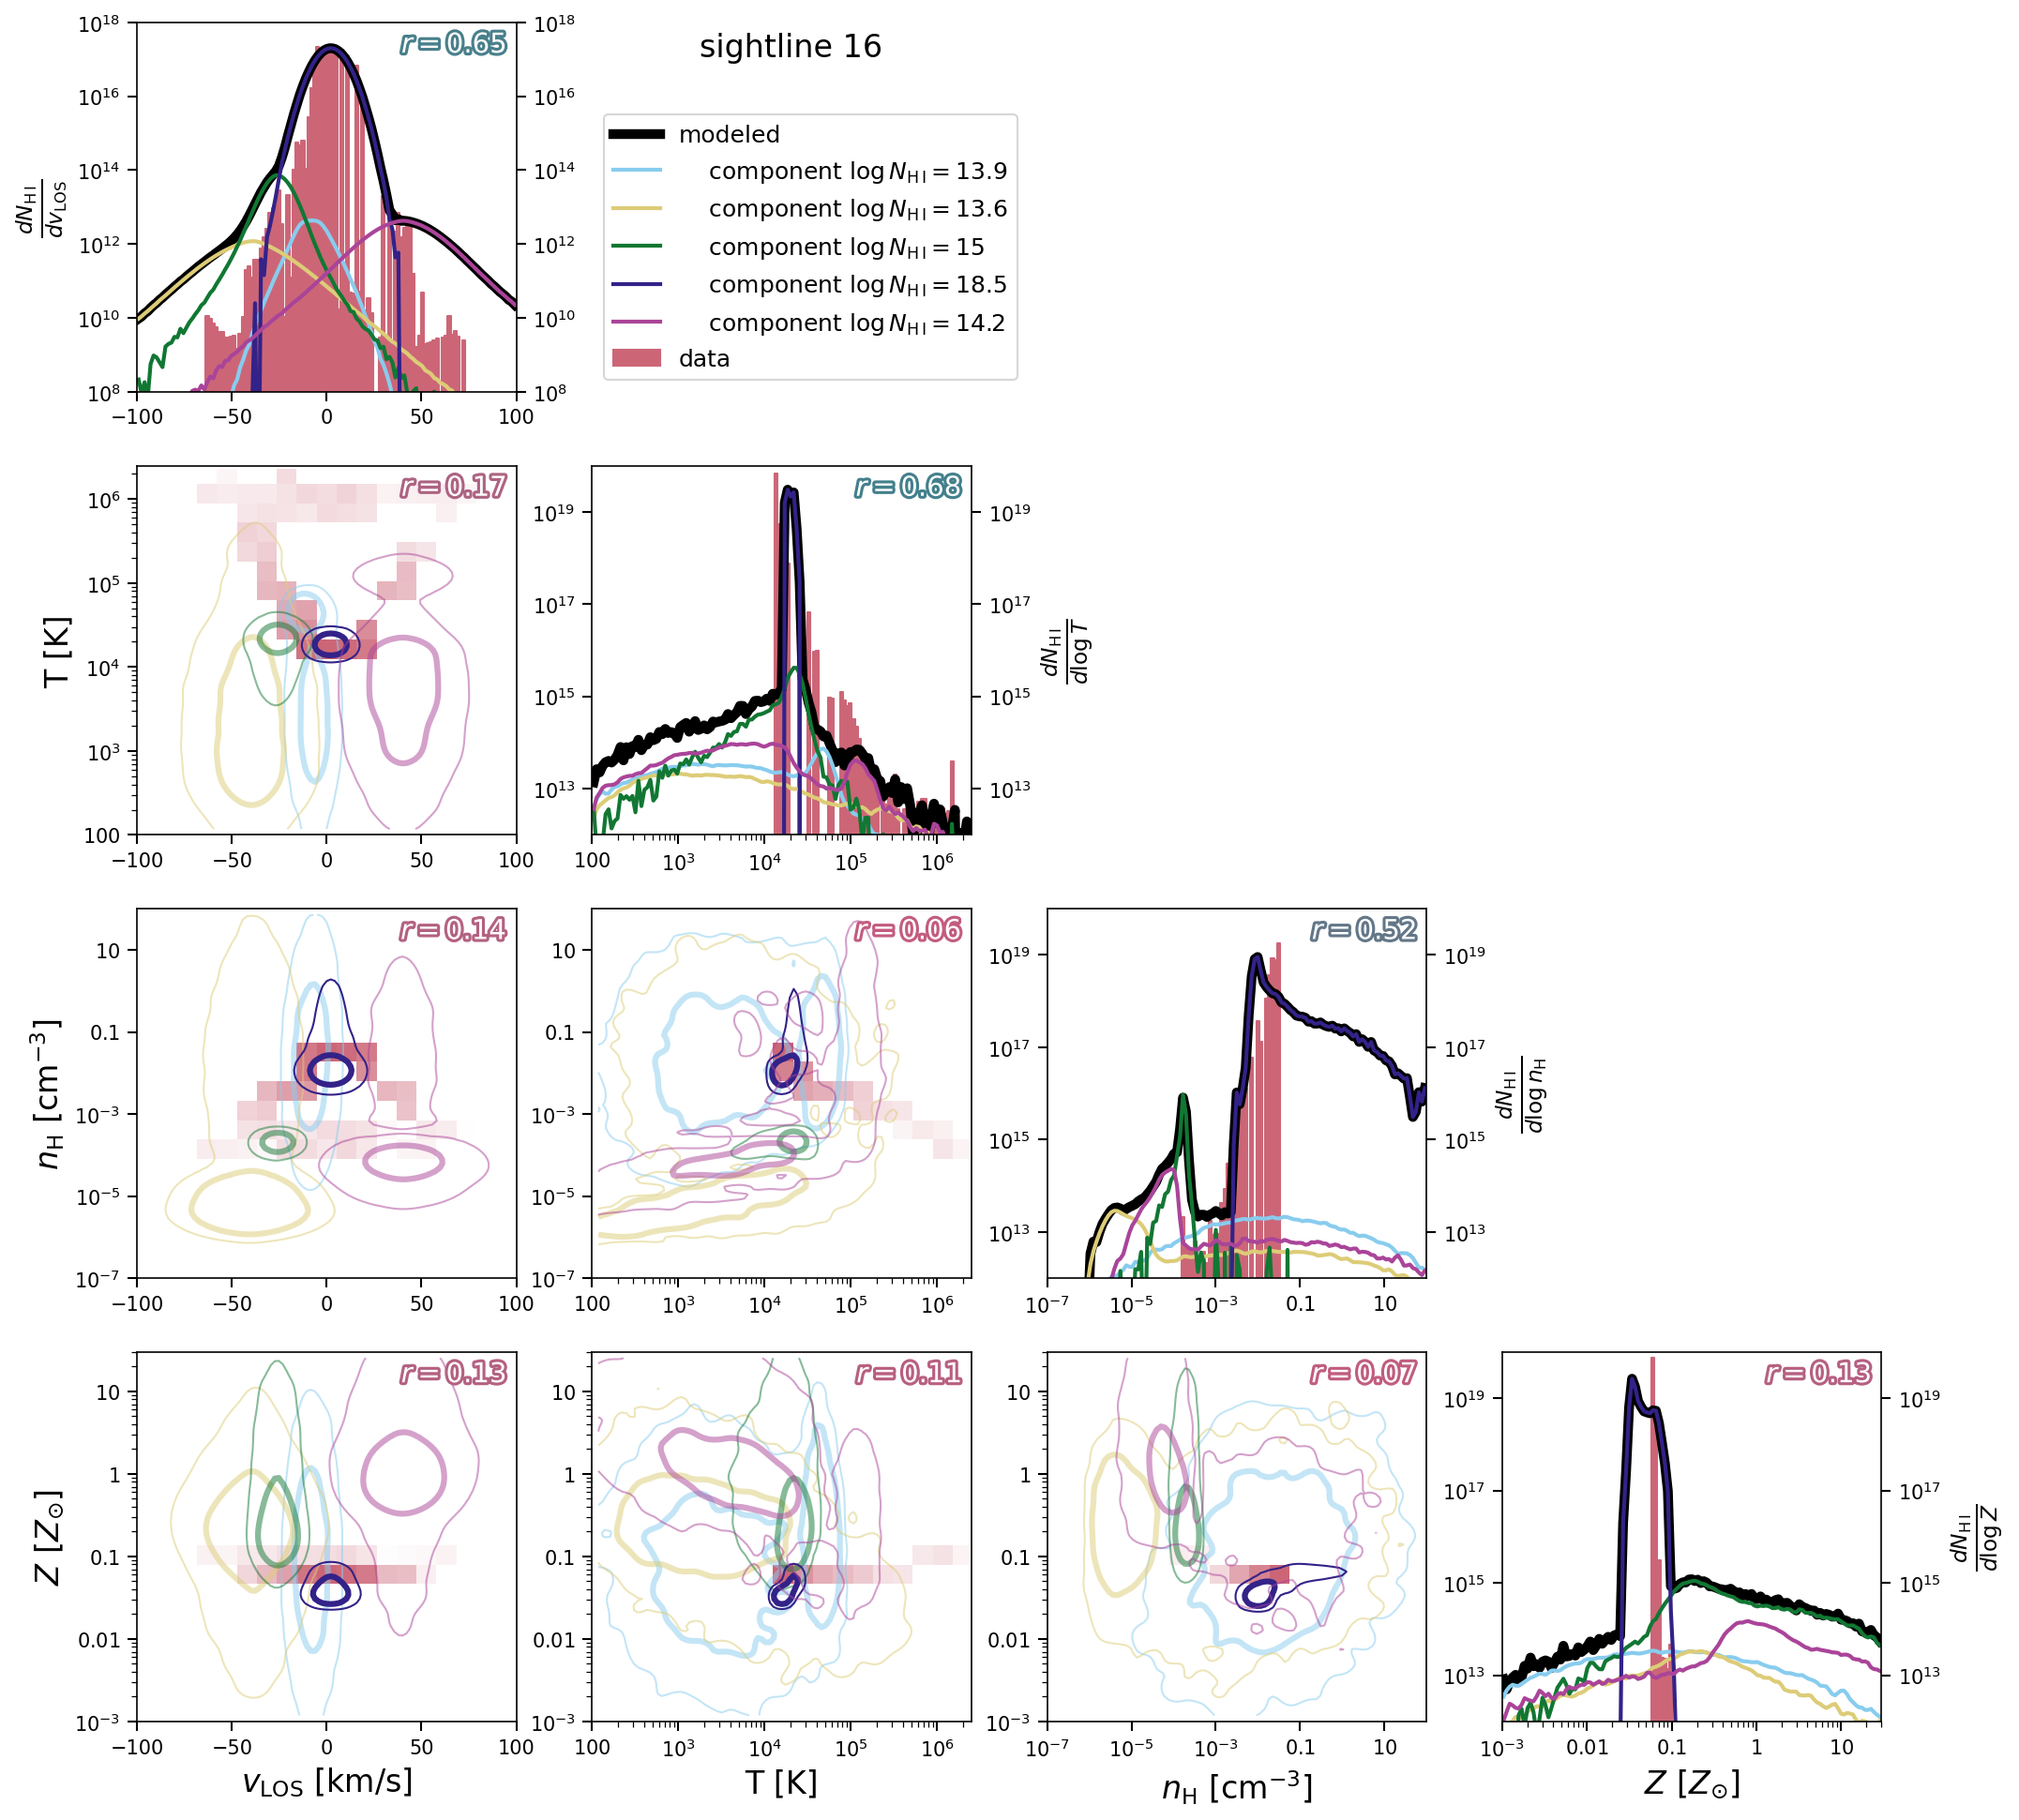
\includegraphics[width=\textwidth]{figures/sample2/sightline_0016.png}
    \label{f: sample2 16}
    \caption{Same as Fig.~\ref{f: sample2 03}, but for sightline 16.}
\end{figure*}

\begin{figure*}
    \centering
    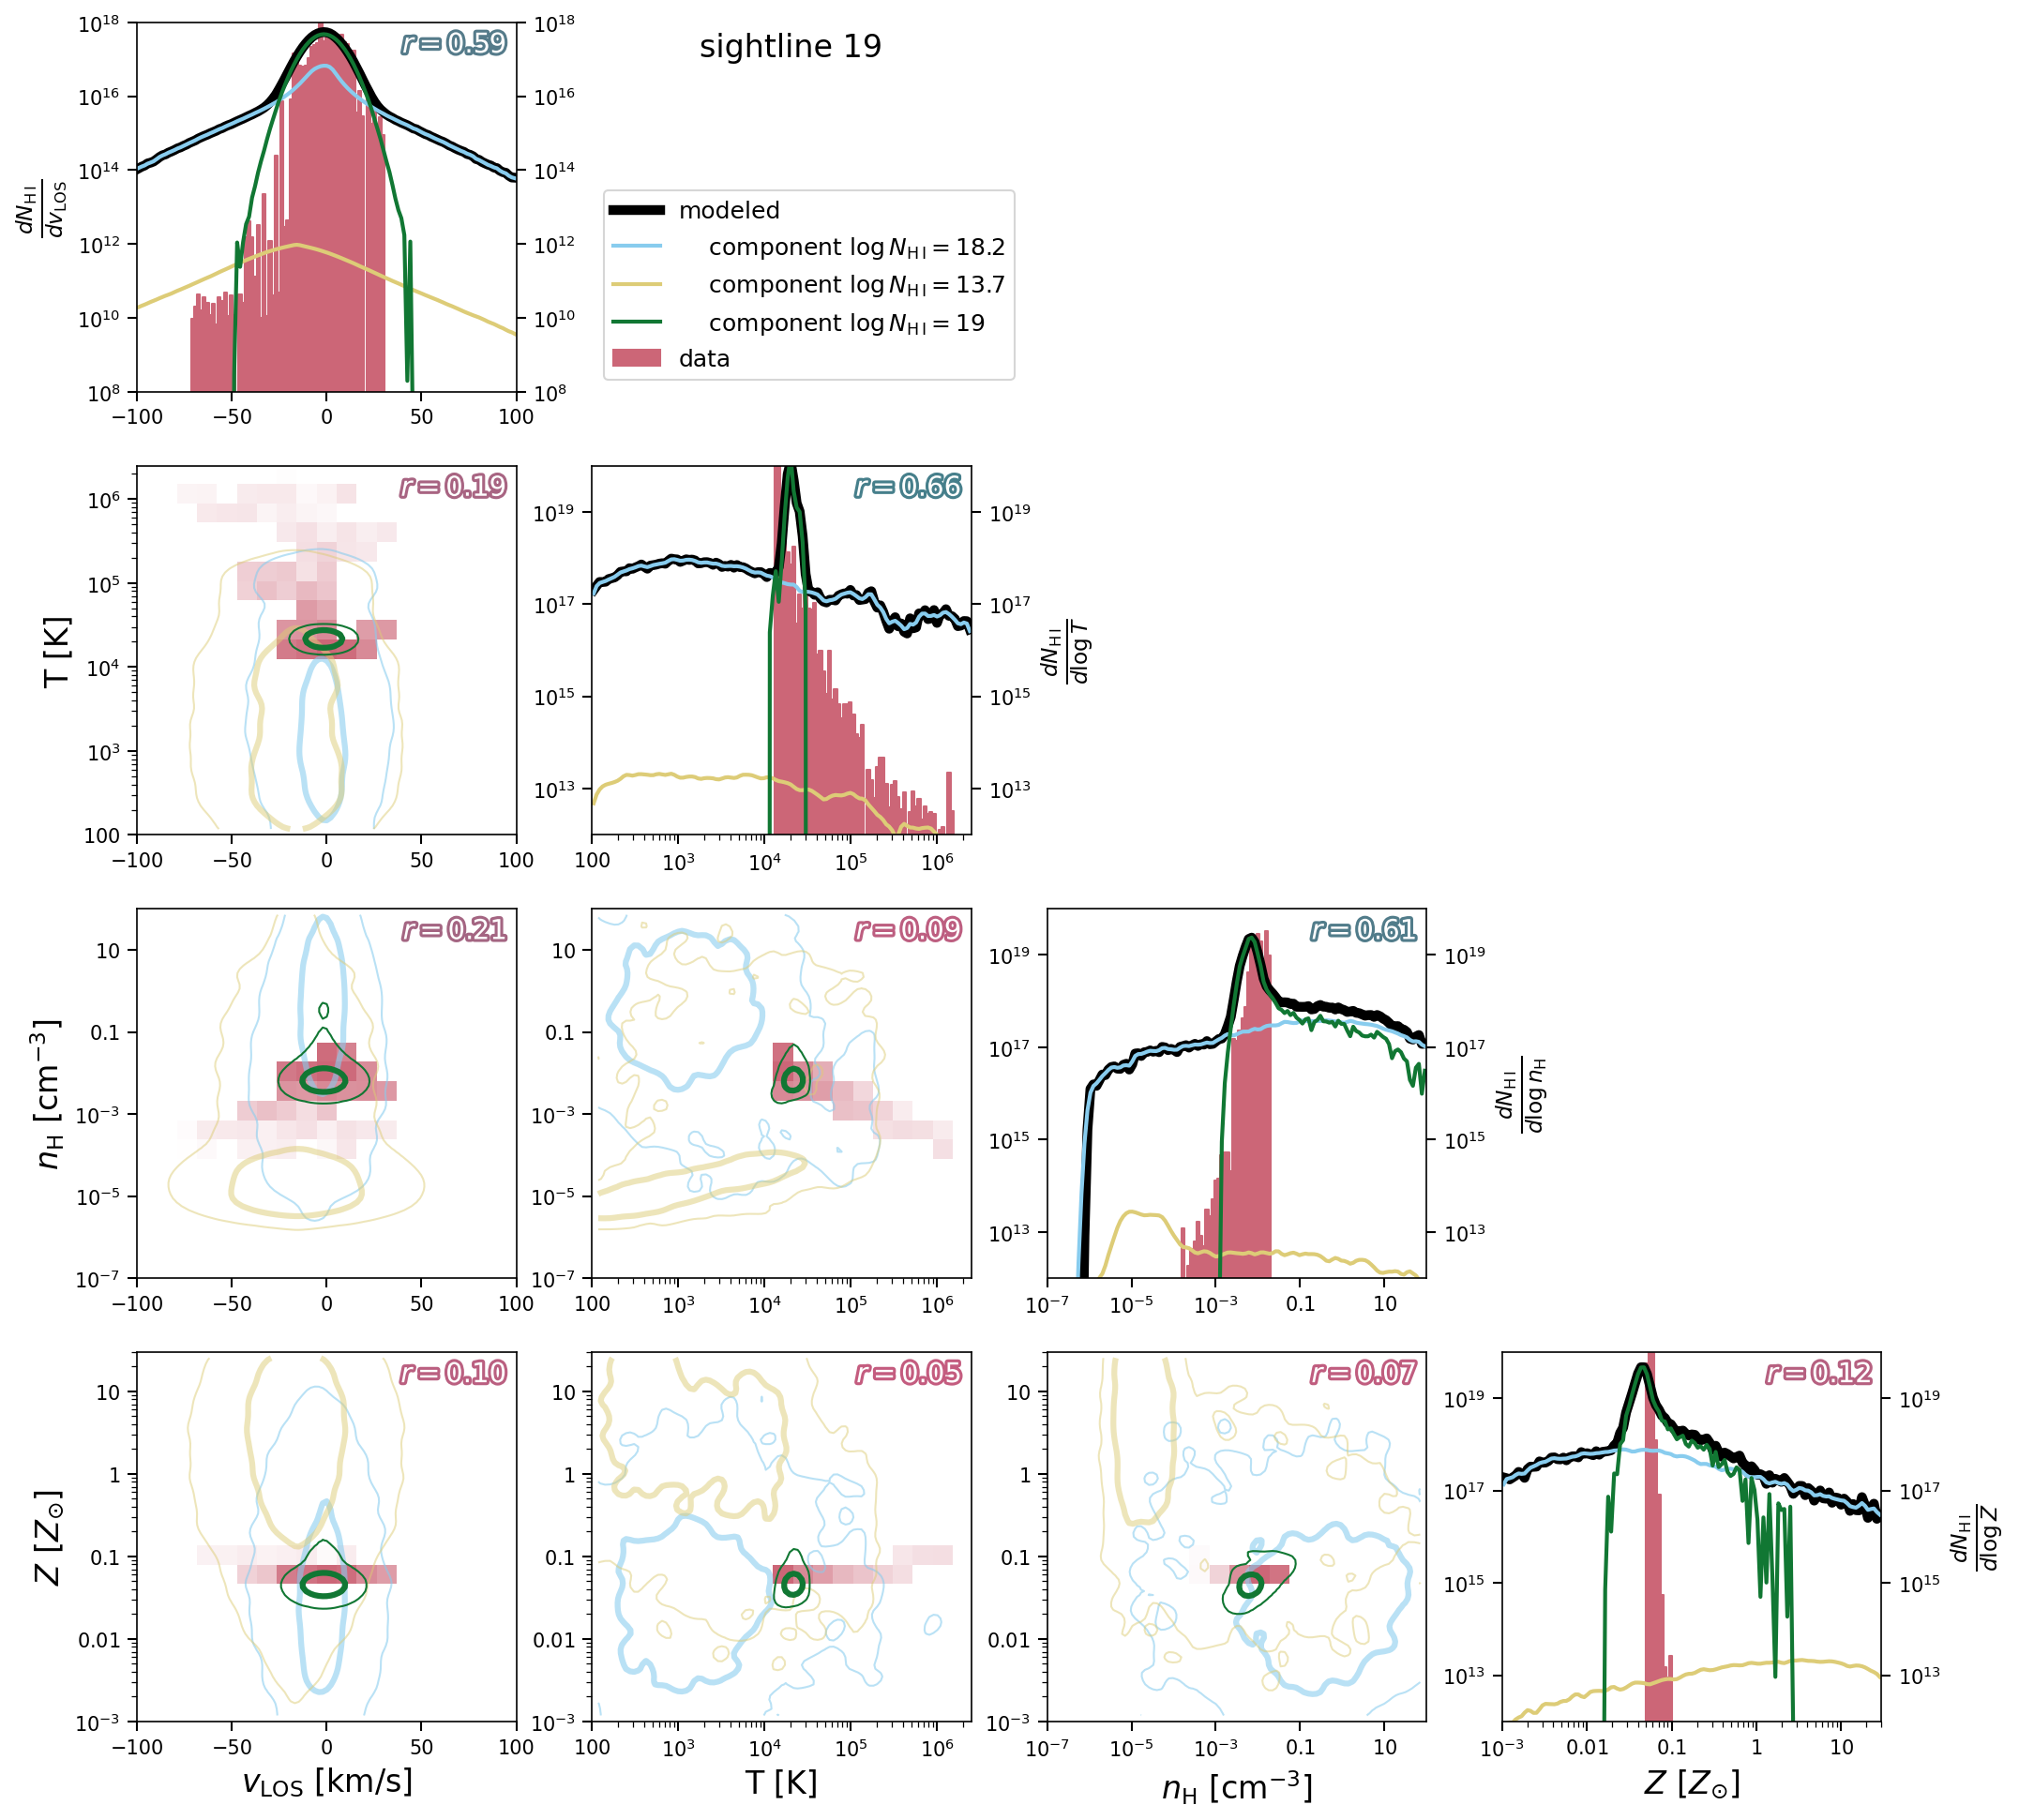
\includegraphics[width=\textwidth]{figures/sample2/sightline_0019.png}
    \label{f: sample2 19}
    \caption{Same as Fig.~\ref{f: sample2 03}, but for sightline 19.}
\end{figure*}

\section{Discussion}

\subsection{What data is required for accurate modeling?}

\todo{What data is necessary in order to get the average properties right?}

\todo{What data is necessary to reproduce the logspace distributions?}

\section{Conclusions}

The last numbered section should briefly summarise what has been done, and describe
the final conclusions which the authors draw from their work.

\section*{Acknowledgements}

The Acknowledgements section is not numbered. Here you can thank helpful
colleagues, acknowledge funding agencies, telescopes and facilities used etc.
Try to keep it short.

%%%%%%%%%%%%%%%%%%%%%%%%%%%%%%%%%%%%%%%%%%%%%%%%%%
\section*{Data Availability}

 
The inclusion of a Data Availability Statement is a requirement for articles published in MNRAS. Data Availability Statements provide a standardised format for readers to understand the availability of data underlying the research results described in the article. The statement may refer to original data generated in the course of the study or to third-party data analysed in the article. The statement should describe and provide means of access, where possible, by linking to the data or providing the required accession numbers for the relevant databases or DOIs.




%%%%%%%%%%%%%%%%%%%% REFERENCES %%%%%%%%%%%%%%%%%%

% The best way to enter references is to use BibTeX:

\bibliographystyle{mnras}
\bibliography{example} % if your bibtex file is called example.bib


% Alternatively you could enter them by hand, like this:
% This method is tedious and prone to error if you have lots of references
%\begin{thebibliography}{99}
%\bibitem[\protect\citeauthoryear{Author}{2012}]{Author2012}
%Author A.~N., 2013, Journal of Improbable Astronomy, 1, 1
%\bibitem[\protect\citeauthoryear{Others}{2013}]{Others2013}
%Others S., 2012, Journal of Interesting Stuff, 17, 198
%\end{thebibliography}

%%%%%%%%%%%%%%%%%%%%%%%%%%%%%%%%%%%%%%%%%%%%%%%%%%

%%%%%%%%%%%%%%%%% APPENDICES %%%%%%%%%%%%%%%%%%%%%

\appendix

\section{Some extra material}

If you want to present additional material which would interrupt the flow of the main paper,
it can be placed in an Appendix which appears after the list of references.

%%%%%%%%%%%%%%%%%%%%%%%%%%%%%%%%%%%%%%%%%%%%%%%%%%


% Don't change these lines
\bsp	% typesetting comment
\label{lastpage}
\end{document}

% End of mnras_template.tex
